% Options for packages loaded elsewhere
\PassOptionsToPackage{unicode}{hyperref}
\PassOptionsToPackage{hyphens}{url}
\documentclass[
]{book}
\usepackage{xcolor}
\usepackage{amsmath,amssymb}
\setcounter{secnumdepth}{-\maxdimen} % remove section numbering
\usepackage{iftex}
\ifPDFTeX
  \usepackage[T1]{fontenc}
  \usepackage[utf8]{inputenc}
  \usepackage{textcomp} % provide euro and other symbols
\else % if luatex or xetex
  \usepackage{unicode-math} % this also loads fontspec
  \defaultfontfeatures{Scale=MatchLowercase}
  \defaultfontfeatures[\rmfamily]{Ligatures=TeX,Scale=1}
\fi
\usepackage{lmodern}
\ifPDFTeX\else
  % xetex/luatex font selection
\fi
% Use upquote if available, for straight quotes in verbatim environments
\IfFileExists{upquote.sty}{\usepackage{upquote}}{}
\IfFileExists{microtype.sty}{% use microtype if available
  \usepackage[]{microtype}
  \UseMicrotypeSet[protrusion]{basicmath} % disable protrusion for tt fonts
}{}
\makeatletter
\@ifundefined{KOMAClassName}{% if non-KOMA class
  \IfFileExists{parskip.sty}{%
    \usepackage{parskip}
  }{% else
    \setlength{\parindent}{0pt}
    \setlength{\parskip}{6pt plus 2pt minus 1pt}}
}{% if KOMA class
  \KOMAoptions{parskip=half}}
\makeatother
\usepackage{graphicx}
\makeatletter
\newsavebox\pandoc@box
\newcommand*\pandocbounded[1]{% scales image to fit in text height/width
  \sbox\pandoc@box{#1}%
  \Gscale@div\@tempa{\textheight}{\dimexpr\ht\pandoc@box+\dp\pandoc@box\relax}%
  \Gscale@div\@tempb{\linewidth}{\wd\pandoc@box}%
  \ifdim\@tempb\p@<\@tempa\p@\let\@tempa\@tempb\fi% select the smaller of both
  \ifdim\@tempa\p@<\p@\scalebox{\@tempa}{\usebox\pandoc@box}%
  \else\usebox{\pandoc@box}%
  \fi%
}
% Set default figure placement to htbp
\def\fps@figure{htbp}
\makeatother
\setlength{\emergencystretch}{3em} % prevent overfull lines
\providecommand{\tightlist}{%
  \setlength{\itemsep}{0pt}\setlength{\parskip}{0pt}}
\usepackage{bookmark}
\IfFileExists{xurl.sty}{\usepackage{xurl}}{} % add URL line breaks if available
\urlstyle{same}
\hypersetup{
  hidelinks,
  pdfcreator={LaTeX via pandoc}}

\author{}
\date{}

\begin{document}
\frontmatter

\mainmatter
\chapter{Menggambar Plot 3D dengan EMT}\label{menggambar-plot-3d-dengan-emt}

Ini adalah pengenalan plot 3D di Euler. Kita memerlukan plot 3D untuk memvisualisasikan fungsi dua variabel.

Euler menggambar fungsi tersebut menggunakan algoritma pengurutan untuk menyembunyikan bagian di latar belakang. Secara umum Euler menggunakan proyeksi pusat. Defaultnya adalah dari kuadran x-y positif menuju titik asal x=y=z=0, tetapi sudut=0° dilihat dari arah sumbu y. Sudut pandang dan ketinggian dapat diubah.

Euler bisa merencanakan

\begin{itemize}
\item
  permukaan dengan garis penetasan dan level atau rentang level,
\item
  awan titik,
\item
  kurva parametrik,
\item
  permukaan implisit.
\end{itemize}

Plot 3D suatu fungsi menggunakan plot3d. Cara termudah adalah dengan memplot ekspresi dalam x dan y. Parameter r mengatur rentang plot sekitar (0,0).

\textgreater aspect(1.5); plot3d(``x\^{}2+sin(y)'',-5,5,0,6*pi):

\begin{figure}
\centering
\pandocbounded{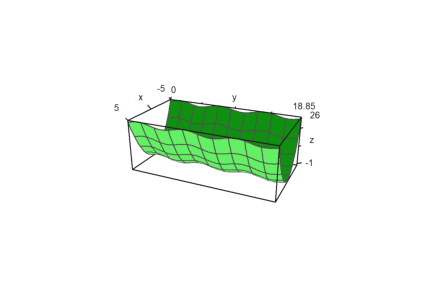
\includegraphics[keepaspectratio]{images/EMT4Plot3D - Naila Khalidatus Salwa-001.png}}
\caption{images/EMT4Plot3D\%20-\%20Naila\%20Khalidatus\%20Salwa-001.png}
\end{figure}

\[x^2+sin(y)\]grafik dari fungsi tersebut seperti pada gambar di atas, -5 dan 5 menunjukkan interval dari sumbu x, sedangkan 0 sampai 6*pi menunjukkan interval sumbu y

\textgreater plot3d(``x\^{}2+x*sin(y)'',-5,5,0,6*pi):

\begin{figure}
\centering
\pandocbounded{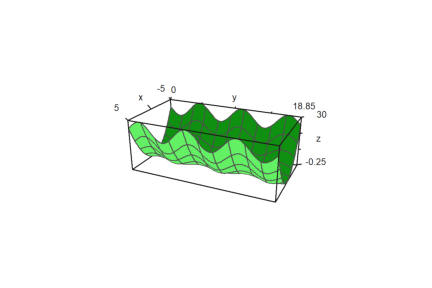
\includegraphics[keepaspectratio]{images/EMT4Plot3D - Naila Khalidatus Salwa-003.png}}
\caption{images/EMT4Plot3D\%20-\%20Naila\%20Khalidatus\%20Salwa-003.png}
\end{figure}

Silakan lakukan modifikasi agar gambar ``talang bergelombang'' tersebut tidak lurus melainkan melengkung/melingkar, baik melingkar secara mendatar maupun melingkar turun/naik (seperti papan peluncur pada kolam renang. Temukan rumusnya.

\textgreater plot3d(``x\^{}2'',-5,5,0,6*pi):

\begin{figure}
\centering
\pandocbounded{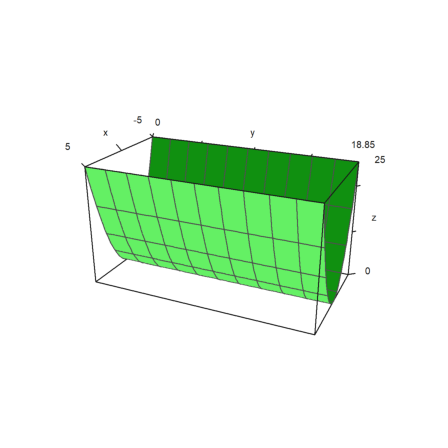
\includegraphics[keepaspectratio]{images/EMT4Plot3D - Naila Khalidatus Salwa-004.png}}
\caption{images/EMT4Plot3D\%20-\%20Naila\%20Khalidatus\%20Salwa-004.png}
\end{figure}

\chapter{Fungsi dua Variabel}\label{fungsi-dua-variabel}

Untuk grafik suatu fungsi, gunakan

\begin{itemize}
\item
  ekspresi sederhana dalam x dan y,
\item
  nama fungsi dari dua variabell
\item
  atau matriks data.
\end{itemize}

Standarnya adalah kisi-kisi kawat berisi dengan warna berbeda di kedua sisi. Perhatikan bahwa jumlah interval kisi default adalah 10, tetapi plot menggunakan jumlah default persegi panjang 40x40 untuk membuat permukaannya. Ini bisa diubah.

\begin{itemize}
\item
  n=40, n={[}40,40{]}: jumlah garis kisi di setiap arah
\item
  grid=10, grid={[}10,10{]}: jumlah garis grid di setiap arah.
\end{itemize}

Kami menggunakan default n=40 dan grid=10.

\textgreater plot3d(``x\textsuperscript{2+y}2''): // plot ini menggunakan n dan grid default

\begin{figure}
\centering
\pandocbounded{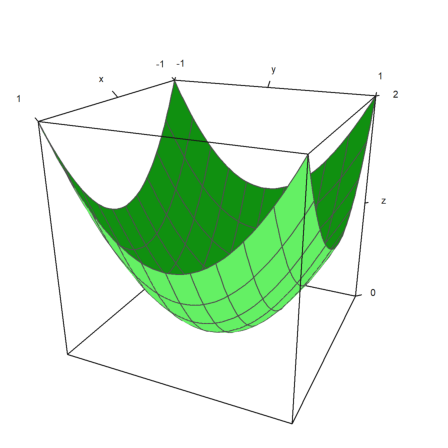
\includegraphics[keepaspectratio]{images/EMT4Plot3D - Naila Khalidatus Salwa-005.png}}
\caption{images/EMT4Plot3D\%20-\%20Naila\%20Khalidatus\%20Salwa-005.png}
\end{figure}

Interaksi pengguna dimungkinkan dengan parameter \textgreater user. Pengguna dapat menekan tombol berikut.

\begin{itemize}
\item
  left,right,up,down: memutar sudut pandang
\item
  +,-: memperbesar atau memperkecil
\item
  a: menghasilkan anaglyph (lihat di bawah)
\item
  l: beralih memutar sumber cahaya (lihat di bawah)
\item
  space: atur ulang ke default
\item
  return: mengakhiri interaksi
\end{itemize}

\textgreater plot3d(``exp(-x\textsuperscript{2+y}2)'',\textgreater user, \ldots{}\\
\textgreater{} title=``Turn with the vector keys (press return to finish)''):

\begin{figure}
\centering
\pandocbounded{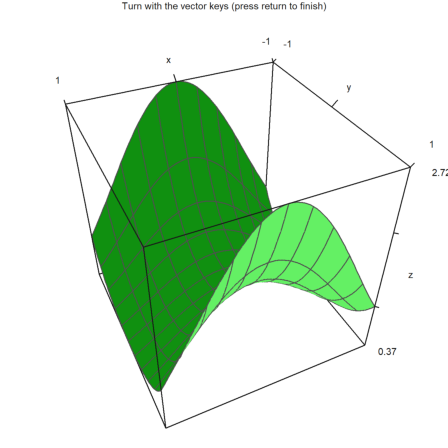
\includegraphics[keepaspectratio]{images/EMT4Plot3D - Naila Khalidatus Salwa-006.png}}
\caption{images/EMT4Plot3D\%20-\%20Naila\%20Khalidatus\%20Salwa-006.png}
\end{figure}

dengan perintah \textgreater user, kita dapat melihat plot dari sudut pandang yang diinginkan

Rentang plot untuk fungsi dapat ditentukan dengan

\begin{itemize}
\item
  a,b: rentang x
\item
  c,d: rentang y
\item
  r: persegi simetris di sekeliling (0,0).
\item
  n: jumlah subinterval untuk plot.
\end{itemize}

Ada beberapa parameter untuk menskalakan fungsi atau mengubah tampilan grafik.

fscale: menskalakan ke nilai fungsi (defaultnya adalah \textless fscale).

scale: angka atau vektor 1x2 untuk menskalakan ke arah x dan y.

frame: jenis bingkai (default 1).

\textgreater plot3d(``exp(-(x\textsuperscript{2+y}2)/5)'',r=10,n=80,fscale=4,scale=1.2,frame=3,\textgreater user):

\begin{figure}
\centering
\pandocbounded{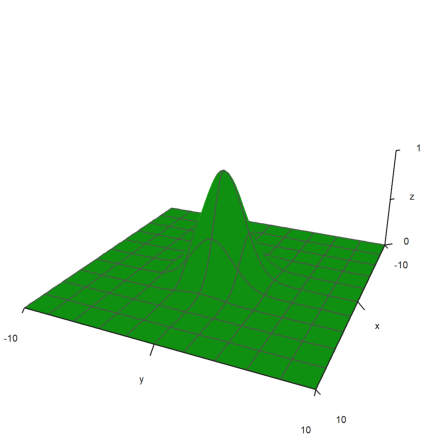
\includegraphics[keepaspectratio]{images/EMT4Plot3D - Naila Khalidatus Salwa-007.png}}
\caption{images/EMT4Plot3D\%20-\%20Naila\%20Khalidatus\%20Salwa-007.png}
\end{figure}

Tampilan dapat diubah dengan berbagai cara.

\begin{itemize}
\item
  distance: jarak pandang ke plot.
\item
  zoom: nilai zoomnya.
\item
  angle: sudut terhadap sumbu y negatif dalam radian.
\item
  height: ketinggian pandangan dalam radian.
\end{itemize}

Nilai default dapat diperiksa atau diubah dengan fungsi view(). Ini mengembalikan parameter dalam urutan di atas.

\textgreater view

\begin{verbatim}
[5,  2.6,  2,  0.4]
\end{verbatim}

Jarak yang lebih dekat membutuhkan lebih sedikit zoom. Efeknya lebih seperti lensa sudut lebar.

Pada contoh berikut, sudut=0 dan tinggi=0 dilihat dari sumbu y negatif. Label sumbu untuk y disembunyikan dalam kasus ini.

\textgreater plot3d(``x\^{}2+y'',distance=3,zoom=1,angle=pi/2,height=0):

\begin{figure}
\centering
\pandocbounded{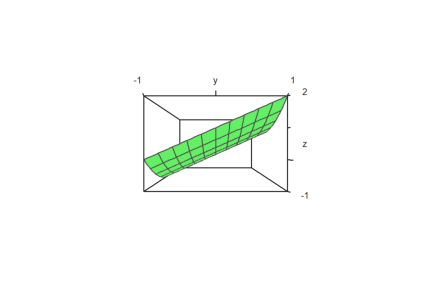
\includegraphics[keepaspectratio]{images/EMT4Plot3D - Naila Khalidatus Salwa-008.png}}
\caption{images/EMT4Plot3D\%20-\%20Naila\%20Khalidatus\%20Salwa-008.png}
\end{figure}

Plot selalu terlihat berada di tengah kubus plot. Anda dapat memindahkan bagian tengah dengan parameter tengah.

\textgreater plot3d(``x\textsuperscript{4+y}2'',a=0,b=1,c=-1,d=1,angle=-20°,height=20°, \ldots{}\\
\textgreater{} center={[}0.4,0,0{]},zoom=5):

\begin{figure}
\centering
\pandocbounded{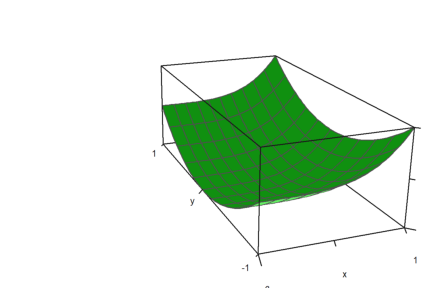
\includegraphics[keepaspectratio]{images/EMT4Plot3D - Naila Khalidatus Salwa-009.png}}
\caption{images/EMT4Plot3D\%20-\%20Naila\%20Khalidatus\%20Salwa-009.png}
\end{figure}

Plot diskalakan agar sesuai dengan unit kubus untuk dilihat. Jadi tidak perlu mengubah jarak atau zoom tergantung ukuran plot. Namun labelnya mengacu pada ukuran sebenarnya.

Jika Anda mematikannya dengan scale=false, Anda harus berhati-hati agar plot tetap masuk ke dalam jendela plotting, dengan mengubah jarak pandang atau zoom, dan memindahkan bagian tengah.

\textgreater plot3d(``5*exp(-x\textsuperscript{2-y}2)'',r=2,\textless fscale,\textless scale,distance=13,height=50°, \ldots{}\\
\textgreater{} center={[}0,0,-2{]},frame=3):

\begin{figure}
\centering
\pandocbounded{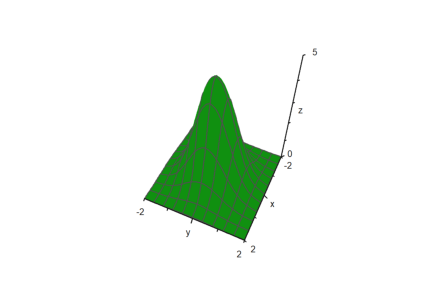
\includegraphics[keepaspectratio]{images/EMT4Plot3D - Naila Khalidatus Salwa-010.png}}
\caption{images/EMT4Plot3D\%20-\%20Naila\%20Khalidatus\%20Salwa-010.png}
\end{figure}

Plot kutub juga tersedia. Parameter polar=true menggambar plot kutub. Fungsi tersebut harus tetap merupakan fungsi dari x dan y. Parameter ``fscale'' menskalakan fungsi dengan skalanya sendiri. Kalau tidak, fungsinya akan diskalakan agar sesuai dengan kubus.

\textgreater plot3d(``1/(x\textsuperscript{2+y}2+1)'',r=5,\textgreater polar, \ldots{}\\
\textgreater{} fscale=2,\textgreater hue,n=100,zoom=4,\textgreater contour,color=blue):

\begin{figure}
\centering
\pandocbounded{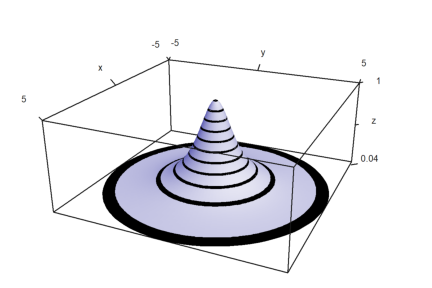
\includegraphics[keepaspectratio]{images/EMT4Plot3D - Naila Khalidatus Salwa-011.png}}
\caption{images/EMT4Plot3D\%20-\%20Naila\%20Khalidatus\%20Salwa-011.png}
\end{figure}

\textgreater function f(r) := exp(-r/2)*cos(r); \ldots{}\\
\textgreater{} plot3d(``f(x\textsuperscript{2+y}2)'',\textgreater polar,scale={[}1,1,0.4{]},r=pi,frame=3,zoom=4):

\begin{figure}
\centering
\pandocbounded{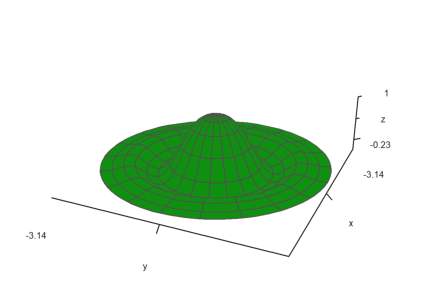
\includegraphics[keepaspectratio]{images/EMT4Plot3D - Naila Khalidatus Salwa-012.png}}
\caption{images/EMT4Plot3D\%20-\%20Naila\%20Khalidatus\%20Salwa-012.png}
\end{figure}

Parameter memutar memutar fungsi di x di sekitar sumbu x.

\begin{itemize}
\item
  rotate=1: Menggunakan sumbu x
\item
  rotate=2: Menggunakan sumbu z
\end{itemize}

\textgreater plot3d(``x\^{}2+1'',a=-1,b=1,rotate=true,grid=5):

\begin{figure}
\centering
\pandocbounded{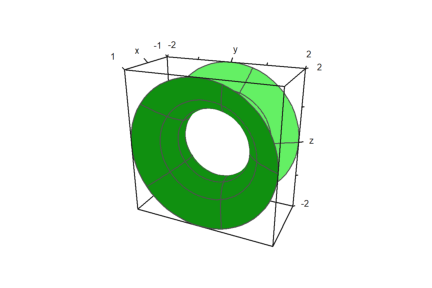
\includegraphics[keepaspectratio]{images/EMT4Plot3D - Naila Khalidatus Salwa-013.png}}
\caption{images/EMT4Plot3D\%20-\%20Naila\%20Khalidatus\%20Salwa-013.png}
\end{figure}

\textgreater plot3d(``x\^{}2+1'',a=-1,b=1,rotate=2,grid=5):

\begin{figure}
\centering
\pandocbounded{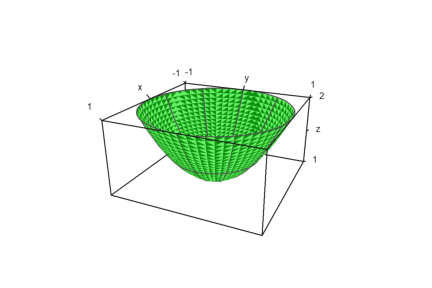
\includegraphics[keepaspectratio]{images/EMT4Plot3D - Naila Khalidatus Salwa-014.png}}
\caption{images/EMT4Plot3D\%20-\%20Naila\%20Khalidatus\%20Salwa-014.png}
\end{figure}

\textgreater plot3d(``sqrt(25-x\^{}2)'',a=0,b=5,rotate=1):

\begin{figure}
\centering
\pandocbounded{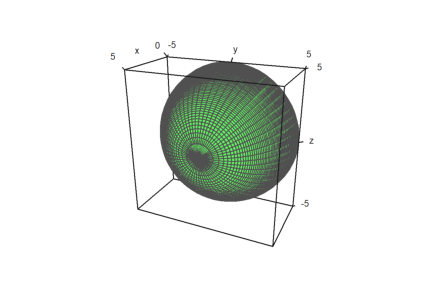
\includegraphics[keepaspectratio]{images/EMT4Plot3D - Naila Khalidatus Salwa-015.png}}
\caption{images/EMT4Plot3D\%20-\%20Naila\%20Khalidatus\%20Salwa-015.png}
\end{figure}

\textgreater{} plot3d(``x*sin(x)'',a=0,b=6pi,rotate=2):

\begin{figure}
\centering
\pandocbounded{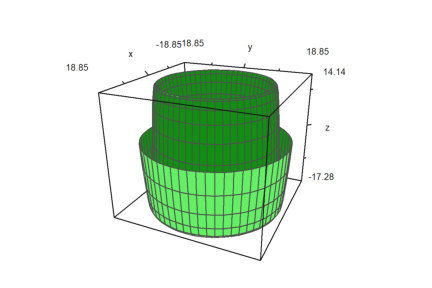
\includegraphics[keepaspectratio]{images/EMT4Plot3D - Naila Khalidatus Salwa-016.png}}
\caption{images/EMT4Plot3D\%20-\%20Naila\%20Khalidatus\%20Salwa-016.png}
\end{figure}

Berikut adalah plot dengan tiga fungsi.

\textgreater plot3d(``x'',``x\textsuperscript{2+y}2'',``y'',r=2,zoom=3.5,frame=3):

\begin{figure}
\centering
\pandocbounded{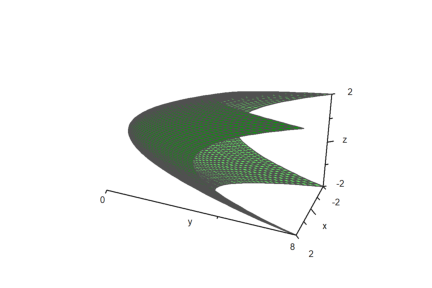
\includegraphics[keepaspectratio]{images/EMT4Plot3D - Naila Khalidatus Salwa-017.png}}
\caption{images/EMT4Plot3D\%20-\%20Naila\%20Khalidatus\%20Salwa-017.png}
\end{figure}

\chapter{Plot Kontur}\label{plot-kontur}

Untuk plotnya, Euler menambahkan garis grid. Sebaliknya dimungkinkan untuk menggunakan garis datar dan rona satu warna atau rona warna spektral. Euler dapat menggambar ketinggian fungsi pada plot dengan arsiran. Di semua plot 3D, Euler dapat menghasilkan anaglyph merah/cyan.

\begin{itemize}
\item
  \textgreater hue: Mengaktifkan bayangan cahaya, bukan kabel.
\item
  \textgreater contour: Membuat plot garis kontur otomatis pada plot.
\item
  level=\ldots{} (or levels): Vektor nilai garis kontur.
\end{itemize}

Standarnya adalah level=``auto'', yang menghitung beberapa garis level secara otomatis. Seperti yang Anda lihat di plot, level sebenarnya adalah rentang level.

Gaya default dapat diubah. Untuk plot kontur berikut, kami menggunakan grid yang lebih halus berukuran 100x100 poin, menskalakan fungsi dan plot, dan menggunakan sudut pandang yang berbeda.

\textgreater plot3d(``exp(-x\textsuperscript{2-y}2)'',r=2,n=100,level=``thin'', \ldots{}\\
\textgreater{} \textgreater contour,\textgreater spectral,fscale=1,scale=1.1,angle=45°,height=20°):

\begin{figure}
\centering
\pandocbounded{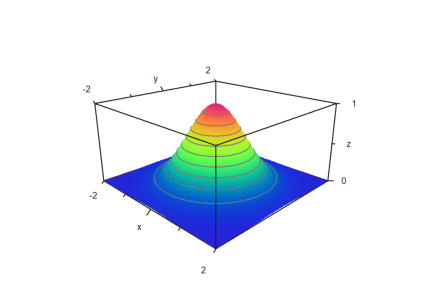
\includegraphics[keepaspectratio]{images/EMT4Plot3D - Naila Khalidatus Salwa-018.png}}
\caption{images/EMT4Plot3D\%20-\%20Naila\%20Khalidatus\%20Salwa-018.png}
\end{figure}

\textgreater plot3d(``exp(x*y)'',angle=100°,\textgreater contour,color=green):

\begin{figure}
\centering
\pandocbounded{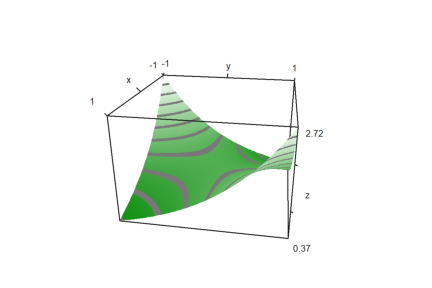
\includegraphics[keepaspectratio]{images/EMT4Plot3D - Naila Khalidatus Salwa-019.png}}
\caption{images/EMT4Plot3D\%20-\%20Naila\%20Khalidatus\%20Salwa-019.png}
\end{figure}

Bayangan defaultnya menggunakan warna abu-abu. Namun rentang warna spektral juga tersedia.

\begin{itemize}
\item
  \textgreater spectral: Menggunakan skema spektral default
\item
  color=\ldots: Menggunakan warna khusus atau skema spektral
\end{itemize}

Untuk plot berikut, kami menggunakan skema spektral default dan menambah jumlah titik untuk mendapatkan tampilan yang sangat mulus.

\textgreater plot3d(``x\textsuperscript{2+y}2'',\textgreater spectral,\textgreater contour,n=100):

\begin{figure}
\centering
\pandocbounded{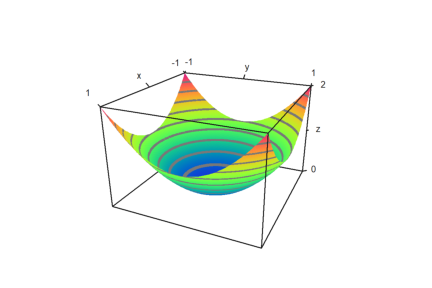
\includegraphics[keepaspectratio]{images/EMT4Plot3D - Naila Khalidatus Salwa-020.png}}
\caption{images/EMT4Plot3D\%20-\%20Naila\%20Khalidatus\%20Salwa-020.png}
\end{figure}

Selain garis level otomatis, kita juga dapat menetapkan nilai garis level. Ini akan menghasilkan garis level yang tipis, bukan rentang level.

\textgreater plot3d(``x\textsuperscript{2-y}2'',0,5,0,5,level=-1:0.1:1,color=redgreen):

\begin{figure}
\centering
\pandocbounded{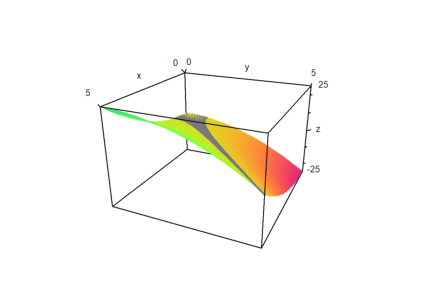
\includegraphics[keepaspectratio]{images/EMT4Plot3D - Naila Khalidatus Salwa-021.png}}
\caption{images/EMT4Plot3D\%20-\%20Naila\%20Khalidatus\%20Salwa-021.png}
\end{figure}

Dalam plot berikut, kita menggunakan dua pita tingkat yang sangat luas dari -0,1 hingga 1, dan dari 0,9 hingga 1. Ini dimasukkan sebagai matriks dengan batas tingkat sebagai kolom.

Selain itu, kami melapisi grid dengan 10 interval di setiap arah.

\textgreater plot3d(``x\textsuperscript{2+y}3'',level={[}-0.1,0.9;0,1{]}, \ldots{}\\
\textgreater{} \textgreater spectral,angle=30°,grid=10,contourcolor=gray):

\begin{figure}
\centering
\pandocbounded{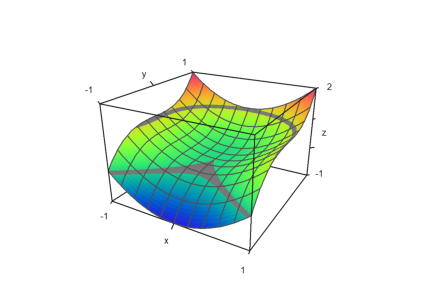
\includegraphics[keepaspectratio]{images/EMT4Plot3D - Naila Khalidatus Salwa-022.png}}
\caption{images/EMT4Plot3D\%20-\%20Naila\%20Khalidatus\%20Salwa-022.png}
\end{figure}

Pada contoh berikut, kita memplot himpunan, di mana

\[f(x,y) = x^y-y^x = 0\]Kami menggunakan satu garis tipis untuk garis level.

\textgreater plot3d(``x\textsuperscript{y-y}x'',level=0,a=0,b=6,c=0,d=6,contourcolor=red,n=100):

\begin{figure}
\centering
\pandocbounded{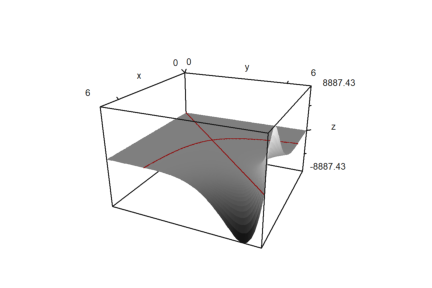
\includegraphics[keepaspectratio]{images/EMT4Plot3D - Naila Khalidatus Salwa-024.png}}
\caption{images/EMT4Plot3D\%20-\%20Naila\%20Khalidatus\%20Salwa-024.png}
\end{figure}

Dimungkinkan untuk menampilkan bidang kontur di bawah plot. Warna dan jarak ke plot dapat ditentukan.

\textgreater plot3d(``x\textsuperscript{2+y}4'',\textgreater cp,cpcolor=green,cpdelta=0.2):

\begin{figure}
\centering
\pandocbounded{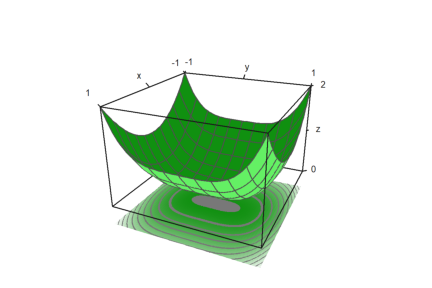
\includegraphics[keepaspectratio]{images/EMT4Plot3D - Naila Khalidatus Salwa-025.png}}
\caption{images/EMT4Plot3D\%20-\%20Naila\%20Khalidatus\%20Salwa-025.png}
\end{figure}

Berikut beberapa gaya lainnya. Kami selalu mematikan bingkai, dan menggunakan berbagai skema warna untuk plot dan kisi.

\textgreater figure(2,2); \ldots{}\\
\textgreater{} expr=``y\textsuperscript{3-x}2''; \ldots{}\\
\textgreater{} figure(1); \ldots{}\\
\textgreater{} plot3d(expr,\textless frame,\textgreater cp,cpcolor=spectral); \ldots{}\\
\textgreater{} figure(2); \ldots{}\\
\textgreater{} plot3d(expr,\textless frame,\textgreater spectral,grid=10,cp=2); \ldots{}\\
\textgreater{} figure(3); \ldots{}\\
\textgreater{} plot3d(expr,\textless frame,\textgreater contour,color=gray,nc=5,cp=3,cpcolor=greenred); \ldots{}\\
\textgreater{} figure(4); \ldots{}\\
\textgreater{} plot3d(expr,\textless frame,\textgreater hue,grid=10,\textgreater transparent,\textgreater cp,cpcolor=gray); \ldots{}\\
\textgreater{} figure(0):

\begin{figure}
\centering
\pandocbounded{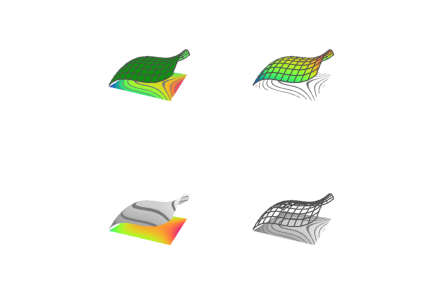
\includegraphics[keepaspectratio]{images/EMT4Plot3D - Naila Khalidatus Salwa-026.png}}
\caption{images/EMT4Plot3D\%20-\%20Naila\%20Khalidatus\%20Salwa-026.png}
\end{figure}

Ada beberapa skema spektral lainnya, yang diberi nomor dari 1 hingga 9. Namun Anda juga dapat menggunakan color=value, di mana nilai

\begin{itemize}
\item
  spectral: untuk rentang dari biru ke merah
\item
  white: untuk rentang yang lebih redup
\item
  yellowblue,purplegreen,blueyellow,greenred
\item
  blueyellow, greenpurple,yellowblue,redgreen
\end{itemize}

\textgreater figure(3,3); \ldots{}\\
\textgreater{} for i=1:9; \ldots{}\\
\textgreater{} figure(i); plot3d(``x\textsuperscript{2+y}2'',spectral=i,\textgreater contour,\textgreater cp,\textless frame,zoom=5); \ldots{}\\
\textgreater{} end; \ldots{}\\
\textgreater{} figure(0):

\begin{figure}
\centering
\pandocbounded{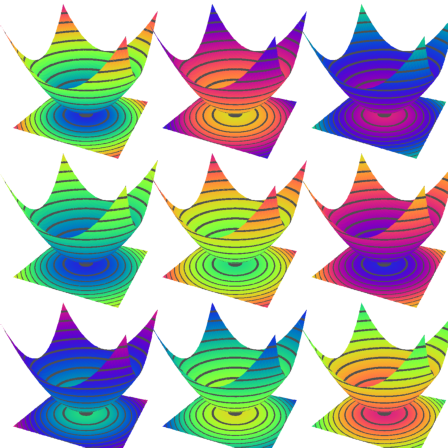
\includegraphics[keepaspectratio]{images/EMT4Plot3D - Naila Khalidatus Salwa-027.png}}
\caption{images/EMT4Plot3D\%20-\%20Naila\%20Khalidatus\%20Salwa-027.png}
\end{figure}

Sumber cahaya dapat diubah dengan l dan tombol kursor selama interaksi pengguna. Itu juga dapat diatur dengan parameter.

\begin{itemize}
\item
  light: arah datangnya cahaya
\item
  amb: cahaya sekitar antara 0 dan 1
\end{itemize}

Perhatikan bahwa program ini tidak membuat perbedaan antara sisi plot. Tidak ada bayangan. Untuk ini, Anda memerlukan Povray.

\textgreater plot3d(``-x\textsuperscript{2-y}2'', \ldots{}\\
\textgreater{} hue=true,light={[}0,1,1{]},amb=0,user=true, \ldots{}\\
\textgreater{} title=``Press l and cursor keys (return to exit)''):

\begin{figure}
\centering
\pandocbounded{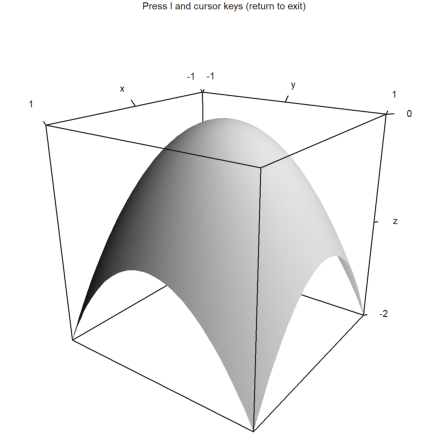
\includegraphics[keepaspectratio]{images/EMT4Plot3D - Naila Khalidatus Salwa-028.png}}
\caption{images/EMT4Plot3D\%20-\%20Naila\%20Khalidatus\%20Salwa-028.png}
\end{figure}

Parameter warna mengubah warna permukaan. Warna garis level juga bisa diubah.

\textgreater plot3d(``-x\textsuperscript{2-y}2'',color=rgb(0.2,0.2,0),hue=true,frame=false, \ldots{}\\
\textgreater{} zoom=3,contourcolor=red,level=-2:0.1:1,dl=0.01):

\begin{figure}
\centering
\pandocbounded{
\includegraphics[keepaspectratio]{images/EMT4Plot3D - Naila Khalidatus Salwa-029.png}}
\caption{images/EMT4Plot3D\%20-\%20Naila\%20Khalidatus\%20Salwa-029.png}
\end{figure}

Warna 0 memberikan efek pelangi yang istimewa.

\textgreater plot3d(``x\textsuperscript{2/(x}2+y\^{}2+1)'',color=0,hue=true,grid=10):

\begin{figure}
\centering
\pandocbounded{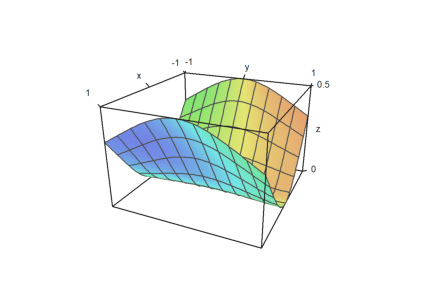
\includegraphics[keepaspectratio]{images/EMT4Plot3D - Naila Khalidatus Salwa-030.png}}
\caption{images/EMT4Plot3D\%20-\%20Naila\%20Khalidatus\%20Salwa-030.png}
\end{figure}

Permukaannya juga bisa transparan.

\textgreater plot3d(``x\textsuperscript{2+y}2'',\textgreater transparent,grid=10,wirecolor=red):

\begin{figure}
\centering
\pandocbounded{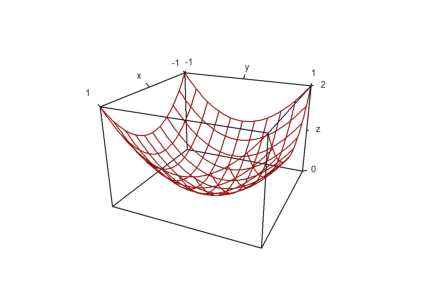
\includegraphics[keepaspectratio]{images/EMT4Plot3D - Naila Khalidatus Salwa-031.png}}
\caption{images/EMT4Plot3D\%20-\%20Naila\%20Khalidatus\%20Salwa-031.png}
\end{figure}

\chapter{Plot Implisit}\label{plot-implisit}

Ada juga plot implisit dalam tiga dimensi. Euler menghasilkan pemotongan melalui objek. Fitur plot3d mencakup plot implisit. Plot ini menunjukkan himpunan nol suatu fungsi dalam tiga variabel.

Solusi dari

\[f(x,y,z) = 0\]dapat divisualisasikan dalam potongan yang sejajar dengan bidang x-y-, x-z- dan y-z.

\begin{itemize}
\item
  implicit=1: memotong sejajar bidang y-z
\item
  implicit=2: memotong sejajar bidang x-z
\item
  implicit=4: memotong sejajar bidang x-y
\end{itemize}

Tambahkan nilai-nilai ini, jika Anda mau. Dalam contoh kita memplot

\[M = \{ (x,y,z) : x^2+y^3+zy=1 \}\]\textgreater plot3d(``x\textsuperscript{2+y}3+z*y-1'',r=5,implicit=3):

\begin{figure}
\centering
\pandocbounded{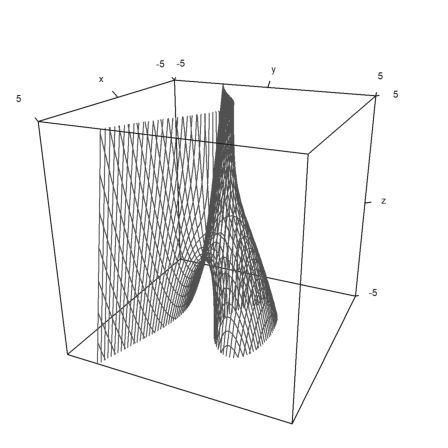
\includegraphics[keepaspectratio]{images/EMT4Plot3D - Naila Khalidatus Salwa-034.png}}
\caption{images/EMT4Plot3D\%20-\%20Naila\%20Khalidatus\%20Salwa-034.png}
\end{figure}

\textgreater c=1; d=1;

\textgreater plot3d(``((x\textsuperscript{2+y}2-c\textsuperscript{2)}2+(z\textsuperscript{2-1)}2)*((y\textsuperscript{2+z}2-c\textsuperscript{2)}2+(x\textsuperscript{2-1)}2)*((z\textsuperscript{2+x}2-c\textsuperscript{2)}2+(y\textsuperscript{2-1)}2)-d'',r=2,\textless frame,\textgreater implicit,\textgreater user):

\begin{figure}
\centering
\pandocbounded{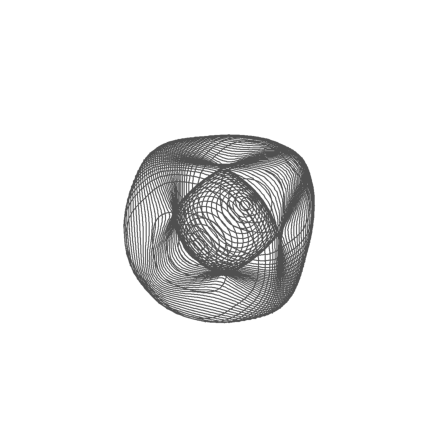
\includegraphics[keepaspectratio]{images/EMT4Plot3D - Naila Khalidatus Salwa-035.png}}
\caption{images/EMT4Plot3D\%20-\%20Naila\%20Khalidatus\%20Salwa-035.png}
\end{figure}

\begin{verbatim}
Cannot combine a 41x41 and a 1x81 matrix for +!
Error in expression: ((x^2+y^2-c^2)^2+(z^2-1)^2)*((y^2+z^2-c^2)^2+(x^2-1)^2)*((z^2+x^2-c^2)^2+(y^2-1)^2)-d
Try "trace errors" to inspect local variables after errors.
pov3d:
    z=f(x,y;args());
\end{verbatim}

\textgreater plot3d(``x\textsuperscript{2+y}2+4*x*z+z\^{}3'',\textgreater implicit,r=2,zoom=2.5):

\begin{figure}
\centering
\pandocbounded{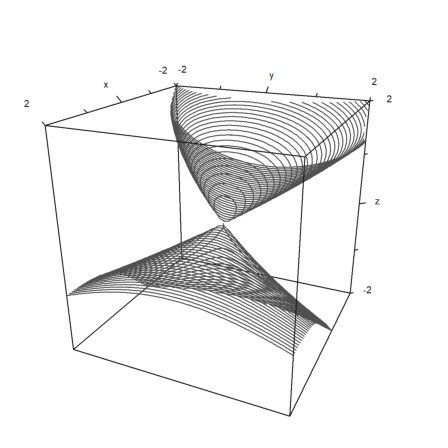
\includegraphics[keepaspectratio]{images/EMT4Plot3D - Naila Khalidatus Salwa-036.png}}
\caption{images/EMT4Plot3D\%20-\%20Naila\%20Khalidatus\%20Salwa-036.png}
\end{figure}

\chapter{Merencanakan Data 3D}\label{merencanakan-data-3d}

Sama seperti plot2d, plot3d menerima data. Untuk objek 3D, Anda perlu menyediakan matriks nilai x-, y- dan z, atau tiga fungsi atau ekspresi fx(x,y), fy(x,y), fz(x,y).

\[\gamma(t,s) = (x(t,s),y(t,s),z(t,s))\]Karena x,y,z adalah matriks, kita asumsikan bahwa (t,s) melewati grid persegi. Hasilnya, Anda dapat memplot gambar persegi panjang di ruang angkasa.

Anda dapat menggunakan bahasa matriks Euler untuk menghasilkan koordinat secara efektif.

Dalam contoh berikut, kita menggunakan vektor nilai t dan vektor kolom nilai s untuk membuat parameter permukaan bola. Dalam gambar kita dapat menandai wilayah, dalam kasus kita wilayah kutub.

\textgreater t=linspace(0,2pi,180); s=linspace(-pi/2,pi/2,90)'; \ldots{}\\
\textgreater{} x=cos(s)*cos(t); y=cos(s)*sin(t); z=sin(s); \ldots{}\\
\textgreater{} plot3d(x,y,z,\textgreater hue, \ldots{}\\
\textgreater{} color=blue,\textless frame,grid={[}10,20{]}, \ldots{}\\
\textgreater{} values=s,contourcolor=red,level={[}90°-24°;90°-22°{]}, \ldots{}\\
\textgreater{} scale=1.4,height=50°):

\begin{figure}
\centering
\pandocbounded{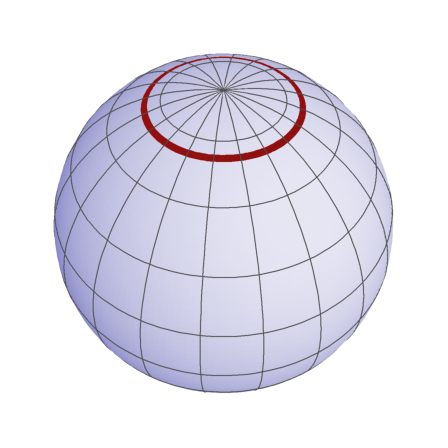
\includegraphics[keepaspectratio]{images/EMT4Plot3D - Naila Khalidatus Salwa-038.png}}
\caption{images/EMT4Plot3D\%20-\%20Naila\%20Khalidatus\%20Salwa-038.png}
\end{figure}

Berikut ini contohnya yaitu grafik suatu fungsi.

\textgreater t=-1:0.1:1; s=(-1:0.1:1)'; plot3d(t,s,t*s,grid=10):

\begin{figure}
\centering
\pandocbounded{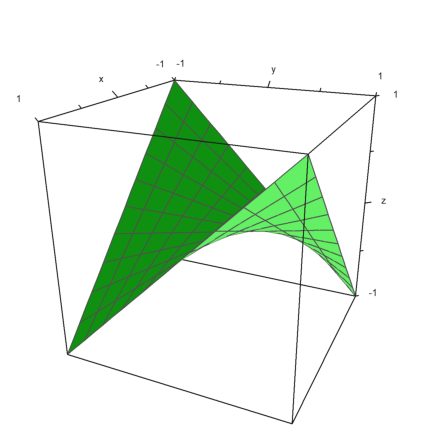
\includegraphics[keepaspectratio]{images/EMT4Plot3D - Naila Khalidatus Salwa-039.png}}
\caption{images/EMT4Plot3D\%20-\%20Naila\%20Khalidatus\%20Salwa-039.png}
\end{figure}

Namun, kita bisa membuat berbagai macam permukaan. Berikut adalah permukaan yang sama sebagai suatu fungsi

\[x = y \, z\]\textgreater plot3d(t*s,t,s,angle=180°,grid=10):

\begin{figure}
\centering
\pandocbounded{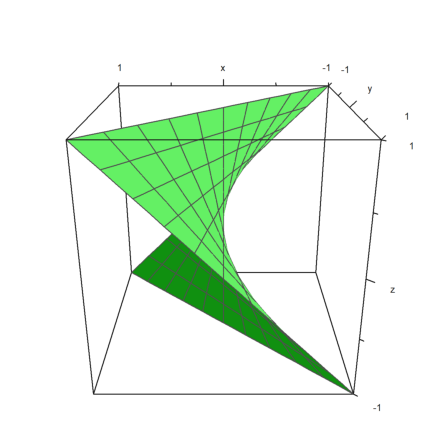
\includegraphics[keepaspectratio]{images/EMT4Plot3D - Naila Khalidatus Salwa-041.png}}
\caption{images/EMT4Plot3D\%20-\%20Naila\%20Khalidatus\%20Salwa-041.png}
\end{figure}

Dengan lebih banyak usaha, kita dapat menghasilkan banyak permukaan.

Dalam contoh berikut kita membuat tampilan bayangan dari bola yang terdistorsi. Koordinat bola yang biasa adalah

\[\gamma(t,s) = (\cos(t)\cos(s),\sin(t)\sin(s),\cos(s))\]dengan

\[0 \le t \le 2\pi, \quad \frac{-\pi}{2} \le s \le \frac{\pi}{2}.\]Kami mendistorsi ini dengan sebuah faktor

\[d(t,s) = \frac{\cos(4t)+\cos(8s)}{4}.\]\textgreater t=linspace(0,2pi,320); s=linspace(-pi/2,pi/2,160)'; \ldots{}\\
\textgreater{} d=1+0.2*(cos(4*t)+cos(8*s)); \ldots{}\\
\textgreater{} plot3d(cos(t)*cos(s)*d,sin(t)*cos(s)*d,sin(s)*d,hue=1, \ldots{}\\
\textgreater{} light={[}1,0,1{]},frame=0,zoom=5):

\begin{figure}
\centering
\pandocbounded{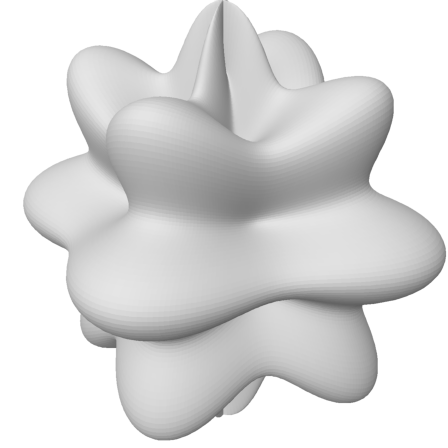
\includegraphics[keepaspectratio]{images/EMT4Plot3D - Naila Khalidatus Salwa-045.png}}
\caption{images/EMT4Plot3D\%20-\%20Naila\%20Khalidatus\%20Salwa-045.png}
\end{figure}

Tentu saja, point cloud juga dimungkinkan. Untuk memplot data titik dalam ruang, kita memerlukan tiga vektor untuk koordinat titik-titik tersebut.

Gayanya sama seperti di plot2d dengan points=true;

\textgreater n=500; \ldots{}\\
\textgreater{} plot3d(normal(1,n),normal(1,n),normal(1,n),points=true,style=``.''):

\begin{figure}
\centering
\pandocbounded{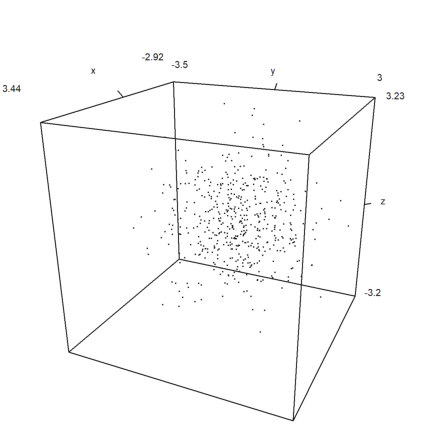
\includegraphics[keepaspectratio]{images/EMT4Plot3D - Naila Khalidatus Salwa-046.png}}
\caption{images/EMT4Plot3D\%20-\%20Naila\%20Khalidatus\%20Salwa-046.png}
\end{figure}

Dimungkinkan juga untuk memplot kurva dalam 3D. Dalam hal ini, lebih mudah untuk menghitung terlebih dahulu titik-titik kurva. Untuk kurva pada bidang kita menggunakan barisan koordinat dan parameter wire=true.

\textgreater t=linspace(0,8pi,500); \ldots{}\\
\textgreater{} plot3d(sin(t),cos(t),t/10,\textgreater wire,zoom=3):

\begin{figure}
\centering
\pandocbounded{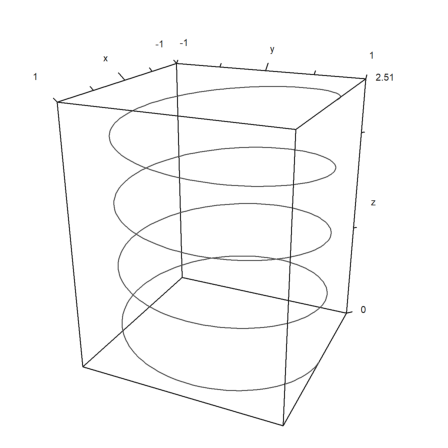
\includegraphics[keepaspectratio]{images/EMT4Plot3D - Naila Khalidatus Salwa-047.png}}
\caption{images/EMT4Plot3D\%20-\%20Naila\%20Khalidatus\%20Salwa-047.png}
\end{figure}

\textgreater t=linspace(0,4pi,1000); plot3d(cos(t),sin(t),t/2pi,\textgreater wire, \ldots{}\\
\textgreater{} linewidth=3,wirecolor=blue):

\begin{figure}
\centering
\pandocbounded{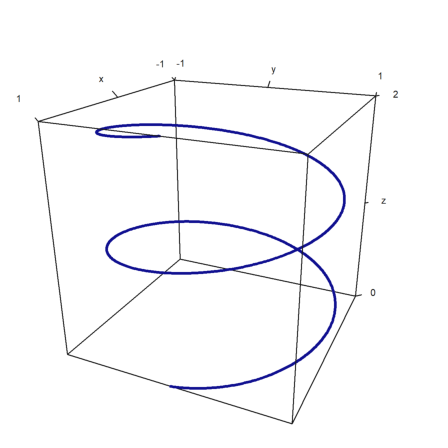
\includegraphics[keepaspectratio]{images/EMT4Plot3D - Naila Khalidatus Salwa-048.png}}
\caption{images/EMT4Plot3D\%20-\%20Naila\%20Khalidatus\%20Salwa-048.png}
\end{figure}

\textgreater X=cumsum(normal(3,100)); \ldots{}\\
\textgreater{} plot3d(X{[}1{]},X{[}2{]},X{[}3{]},\textgreater anaglyph,\textgreater wire):

\begin{figure}
\centering
\pandocbounded{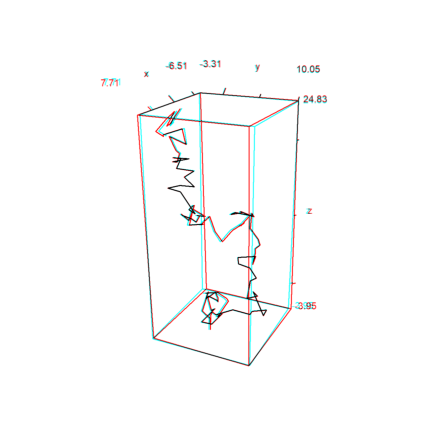
\includegraphics[keepaspectratio]{images/EMT4Plot3D - Naila Khalidatus Salwa-049.png}}
\caption{images/EMT4Plot3D\%20-\%20Naila\%20Khalidatus\%20Salwa-049.png}
\end{figure}

EMT juga dapat membuat plot dalam mode anaglyph. Untuk melihat plot seperti itu, Anda memerlukan kacamata berwarna merah/sian.

\textgreater{} plot3d(``x\textsuperscript{2+y}3'',\textgreater anaglyph,\textgreater contour,angle=30°):

\begin{figure}
\centering
\pandocbounded{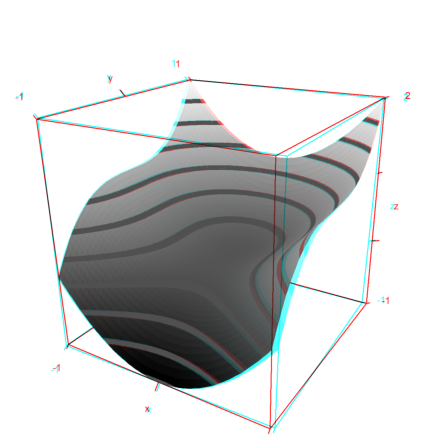
\includegraphics[keepaspectratio]{images/EMT4Plot3D - Naila Khalidatus Salwa-050.png}}
\caption{images/EMT4Plot3D\%20-\%20Naila\%20Khalidatus\%20Salwa-050.png}
\end{figure}

Seringkali skema warna spektral digunakan untuk plot. Ini menekankan ketinggian fungsinya.

\textgreater plot3d(``x\textsuperscript{2*y}3-y'',\textgreater spectral,\textgreater contour,zoom=3.2):

\begin{figure}
\centering
\pandocbounded{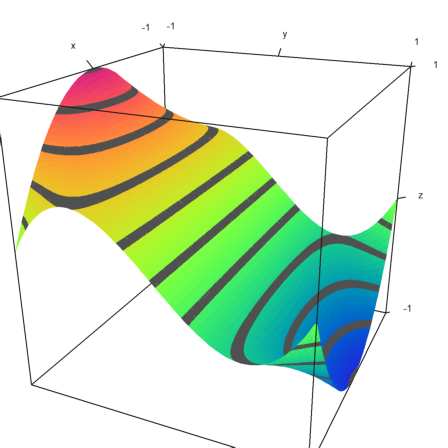
\includegraphics[keepaspectratio]{images/EMT4Plot3D - Naila Khalidatus Salwa-051.png}}
\caption{images/EMT4Plot3D\%20-\%20Naila\%20Khalidatus\%20Salwa-051.png}
\end{figure}

Euler juga dapat memplot permukaan yang diparameterisasi, jika parameternya adalah nilai x, y, dan z dari gambar kotak persegi panjang di ruang tersebut.

Untuk demo berikut, kami menyiapkan parameter u- dan v-, dan menghasilkan koordinat ruang dari parameter tersebut.

\textgreater u=linspace(-1,1,10); v=linspace(0,2*pi,50)'; \ldots{}\\
\textgreater{} X=(3+u*cos(v/2))*cos(v); Y=(3+u*cos(v/2))*sin(v); Z=u*sin(v/2); \ldots{}\\
\textgreater{} plot3d(X,Y,Z,\textgreater anaglyph,\textless frame,\textgreater wire,scale=2.3):

\begin{figure}
\centering
\pandocbounded{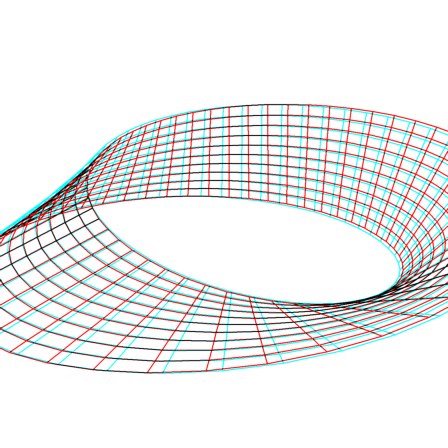
\includegraphics[keepaspectratio]{images/EMT4Plot3D - Naila Khalidatus Salwa-052.png}}
\caption{images/EMT4Plot3D\%20-\%20Naila\%20Khalidatus\%20Salwa-052.png}
\end{figure}

Berikut adalah contoh yang lebih rumit, yang megah dengan kacamata merah/cyan.

\textgreater u:=linspace(-pi,pi,160); v:=linspace(-pi,pi,400)'; \ldots{}\\
\textgreater{} x:=(4*(1+.25*sin(3*v))+cos(u))*cos(2*v); \ldots{}\\
\textgreater{} y:=(4*(1+.25*sin(3*v))+cos(u))*sin(2*v); \ldots{}\\
\textgreater{} z=sin(u)+2*cos(3*v); \ldots{}\\
\textgreater{} plot3d(x,y,z,frame=0,scale=1.5,hue=1,light={[}1,0,-1{]},zoom=2.8,\textgreater anaglyph):

\begin{figure}
\centering
\pandocbounded{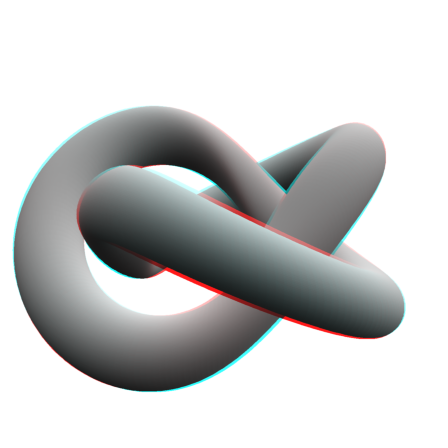
\includegraphics[keepaspectratio]{images/EMT4Plot3D - Naila Khalidatus Salwa-053.png}}
\caption{images/EMT4Plot3D\%20-\%20Naila\%20Khalidatus\%20Salwa-053.png}
\end{figure}

\chapter{Plot Statistik}\label{plot-statistik}

Plot batang juga dimungkinkan. Untuk itu, kita harus menyediakannya

\begin{itemize}
\item
  x: vektor baris dengan n+1 elemen, mewakili posisi di sumbu x
\item
  y: vektor kolom dengan n+1 elemen, mewakili posisi di sumbu y
\item
  z: matriks dengan nilai nxn, mewakili tinggi batang
\end{itemize}

z bisa lebih besar, tetapi hanya nilai nxn yang akan digunakan.

Dalam contoh ini, pertama-tama kita menghitung nilainya. Kemudian kita sesuaikan x dan y, sehingga vektor-vektornya berpusat pada nilai yang digunakan.

\textgreater x=-1:0.1:1; y=x'; z=x\textsuperscript{2+y}2; \ldots{}\\
\textgreater{} xa=(x\textbar1.1)-0.05; ya=(y\_1.1)-0.05; \ldots{}\\
\textgreater{} plot3d(xa,ya,z,bar=true):

\begin{figure}
\centering
\pandocbounded{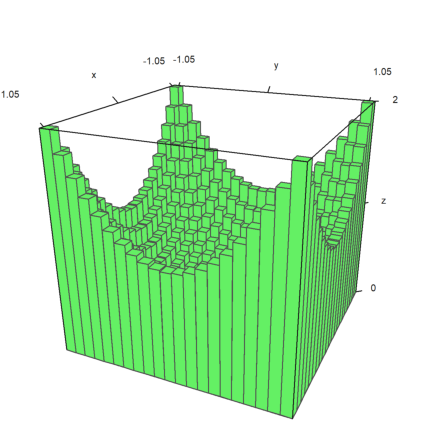
\includegraphics[keepaspectratio]{images/EMT4Plot3D - Naila Khalidatus Salwa-054.png}}
\caption{images/EMT4Plot3D\%20-\%20Naila\%20Khalidatus\%20Salwa-054.png}
\end{figure}

\textgreater{}

Dimungkinkan untuk membagi plot suatu permukaan menjadi dua bagian atau lebih.

\textgreater x=-1:0.1:1; y=x'; z=x+y; d=zeros(size(x)); \ldots{}\\
\textgreater{} plot3d(x,y,z,disconnect=2:2:20):

\begin{figure}
\centering
\pandocbounded{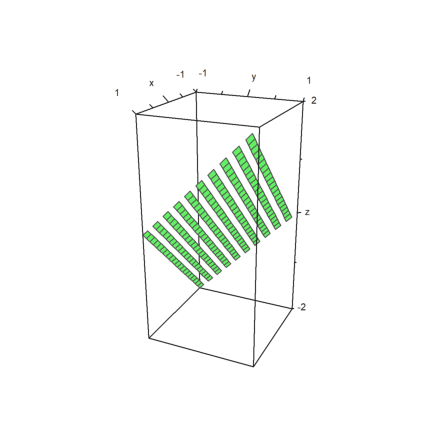
\includegraphics[keepaspectratio]{images/EMT4Plot3D - Naila Khalidatus Salwa-055.png}}
\caption{images/EMT4Plot3D\%20-\%20Naila\%20Khalidatus\%20Salwa-055.png}
\end{figure}

Jika memuat atau menghasilkan matriks data M dari file dan perlu memplotnya dalam 3D, Anda dapat menskalakan matriks ke {[}-1,1{]} dengan skala(M), atau menskalakan matriks dengan \textgreater zscale. Hal ini dapat dikombinasikan dengan faktor penskalaan individual yang diterapkan sebagai tambahan.

\textgreater i=1:20; j=i'; \ldots{}\\
\textgreater{} plot3d(i*j\^{}2+100*normal(20,20),\textgreater zscale,scale={[}1,1,1.5{]},angle=-40°,zoom=1.8):

\begin{figure}
\centering
\pandocbounded{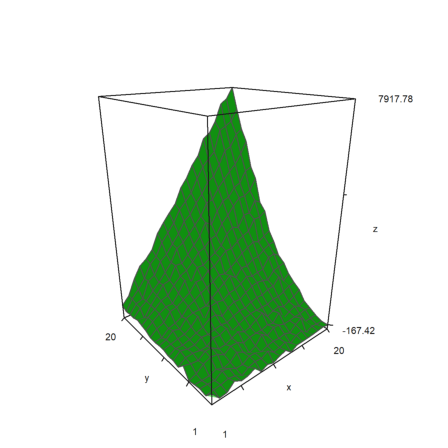
\includegraphics[keepaspectratio]{images/EMT4Plot3D - Naila Khalidatus Salwa-056.png}}
\caption{images/EMT4Plot3D\%20-\%20Naila\%20Khalidatus\%20Salwa-056.png}
\end{figure}

\textgreater Z=intrandom(5,100,6); v=zeros(5,6); \ldots{}\\
\textgreater{} loop 1 to 5; v{[}\#{]}=getmultiplicities(1:6,Z{[}\#{]}); end; \ldots{}\\
\textgreater{} columnsplot3d(v',scols=1:5,ccols={[}1:5{]}):

\begin{figure}
\centering
\pandocbounded{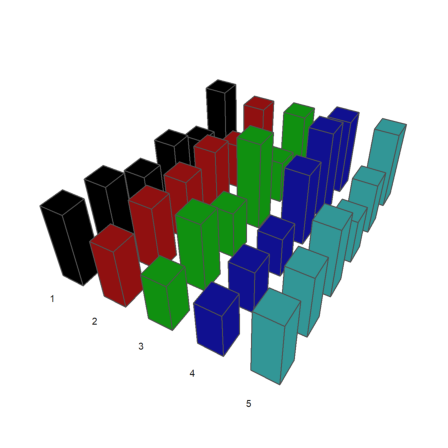
\includegraphics[keepaspectratio]{images/EMT4Plot3D - Naila Khalidatus Salwa-057.png}}
\caption{images/EMT4Plot3D\%20-\%20Naila\%20Khalidatus\%20Salwa-057.png}
\end{figure}

intandom = membuat plot dengan banyaknya baris dan kolom yang sudah ditentukan dengan nilai-nilai matriksnya bilangan bulat acak

\chapter{Permukaan Benda Putar}\label{permukaan-benda-putar}

\textgreater plot2d(``(x\textsuperscript{2+y}2-1)\textsuperscript{3-x}2*y\^{}3'',r=1.3, \ldots{}\\
\textgreater{} style=``\#'',color=red,\textless outline, \ldots{}\\
\textgreater{} level={[}-2;0{]},n=100):

\begin{figure}
\centering
\pandocbounded{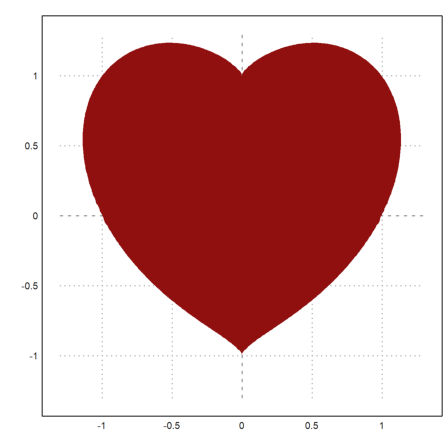
\includegraphics[keepaspectratio]{images/EMT4Plot3D - Naila Khalidatus Salwa-058.png}}
\caption{images/EMT4Plot3D\%20-\%20Naila\%20Khalidatus\%20Salwa-058.png}
\end{figure}

\textgreater ekspresi \&= (x\textsuperscript{2+y}2-1)\textsuperscript{3-x}2*y\^{}3; \$ekspresi

\[\left(y^2+x^2-1\right)^3-x^2\,y^3\]Kami ingin memutar kurva hati di sekitar sumbu y. Inilah ekspresi yang mendefinisikan hati:

\[f(x,y)=(x^2+y^2-1)^3-x^2.y^3.\]Selanjutnya kita atur

\[x=r.cos(a),\quad y=r.sin(a).\]\textgreater function fr(r,a) \&= ekspresi with {[}x=r*cos(a),y=r*sin(a){]} \textbar{} trigreduce; \$fr(r,a)

\[\left(r^2-1\right)^3+\frac{\left(\sin \left(5\,a\right)-\sin \left(  3\,a\right)-2\,\sin a\right)\,r^5}{16}\]Hal ini memungkinkan untuk mendefinisikan fungsi numerik, yang menyelesaikan r, jika a diberikan. Dengan fungsi tersebut kita dapat memplot heart yang diputar sebagai permukaan parametrik.

\textgreater function map f(a) := bisect(``fr'',0,2;a); \ldots{}\\
\textgreater{} t=linspace(-pi/2,pi/2,100); r=f(t); \ldots{}\\
\textgreater{} s=linspace(pi,2pi,100)'; \ldots{}\\
\textgreater{} plot3d(r*cos(t)*sin(s),r*cos(t)*cos(s),r*sin(t), \ldots{}\\
\textgreater{} \textgreater hue,\textless frame,color=red,zoom=4,amb=0,max=0.7,grid=12,height=50°):

\begin{figure}
\centering
\pandocbounded{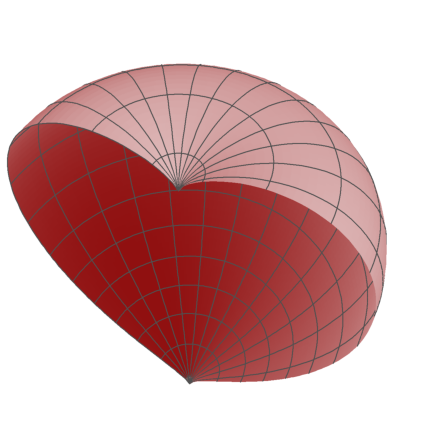
\includegraphics[keepaspectratio]{images/EMT4Plot3D - Naila Khalidatus Salwa-063.png}}
\caption{images/EMT4Plot3D\%20-\%20Naila\%20Khalidatus\%20Salwa-063.png}
\end{figure}

Berikut ini adalah plot 3D dari gambar di atas yang diputar mengelilingi sumbu z. Kami mendefinisikan fungsi yang mendeskripsikan objek.

\textgreater function f(x,y,z) \ldots{}

\begin{verbatim}
r=x^2+y^2;
return (r+z^2-1)^3-r*z^3;
 endfunction
\end{verbatim}

\textgreater plot3d(``f(x,y,z)'', \ldots{}\\
\textgreater{} xmin=0,xmax=1.2,ymin=-1.2,ymax=1.2,zmin=-1.2,zmax=1.4, \ldots{}\\
\textgreater{} implicit=1,angle=-30°,zoom=2.5,n={[}10,100,60{]},\textgreater anaglyph):

\begin{figure}
\centering
\pandocbounded{\includegraphics[keepaspectratio]{images/EMT4Plot3D - Naila Khalidatus Salwa-064.png}}
\caption{images/EMT4Plot3D\%20-\%20Naila\%20Khalidatus\%20Salwa-064.png}
\end{figure}

\chapter{Plot 3D Khusus}\label{plot-3d-khusus}

Fungsi plot3d bagus untuk dimiliki, tetapi tidak memenuhi semua kebutuhan. Selain rutinitas yang lebih mendasar, dimungkinkan untuk mendapatkan plot berbingkai dari objek apa pun yang Anda suka.

Meskipun Euler bukan program 3D, ia dapat menggabungkan beberapa objek dasar. Kami mencoba memvisualisasikan paraboloid dan garis singgungnya.

\textgreater function myplot \ldots{}

\begin{verbatim}
  y=-1:0.01:1; x=(-1:0.01:1)';
  plot3d(x,y,0.2*(x-0.1)/2,<scale,<frame,>hue, ..
    hues=0.5,>contour,color=orange);
  h=holding(1);
  plot3d(x,y,(x^2+y^2)/2,<scale,<frame,>contour,>hue);
  holding(h);
endfunction
\end{verbatim}

Sekarang framedplot() menyediakan bingkai, dan mengatur tampilan.

\textgreater framedplot(``myplot'',{[}-1,1,-1,1,0,1{]},height=0,angle=-30°, \ldots{}\\
\textgreater{} center={[}0,0,-0.7{]},zoom=3):

\begin{figure}
\centering
\pandocbounded{\includegraphics[keepaspectratio]{images/EMT4Plot3D - Naila Khalidatus Salwa-065.png}}
\caption{images/EMT4Plot3D\%20-\%20Naila\%20Khalidatus\%20Salwa-065.png}
\end{figure}

Dengan cara yang sama, Anda dapat memplot bidang kontur secara manual. Perhatikan bahwa plot3d() menyetel jendela ke fullwindow() secara default, tetapi plotcontourplane() berasumsi demikian.

\textgreater x=-1:0.02:1.1; y=x'; z=x\textsuperscript{2-y}4;

\textgreater function myplot (x,y,z) \ldots{}\\
\textgreater{}\\

\textgreater myplot(x,y,z):

\begin{figure}
\centering
\pandocbounded{\includegraphics[keepaspectratio]{images/EMT4Plot3D - Naila Khalidatus Salwa-066.png}}
\caption{images/EMT4Plot3D\%20-\%20Naila\%20Khalidatus\%20Salwa-066.png}
\end{figure}

\chapter{Animasi}\label{animasi}

Euler dapat menggunakan frame untuk melakukan pra-komputasi animasi.

Salah satu fungsi yang memanfaatkan teknik ini adalah memutar. Itu dapat mengubah sudut pandang dan menggambar ulang plot 3D. Fungsi ini memanggil addpage() untuk setiap plot baru. Akhirnya ia menganimasikan plotnya.

Silakan pelajari sumber rotasi untuk melihat lebih detail.

\textgreater function testplot () := plot3d(``x\textsuperscript{2+y}3''); \ldots{}\\
\textgreater{} rotate(``testplot''); testplot():

\begin{figure}
\centering
\pandocbounded{\includegraphics[keepaspectratio]{images/EMT4Plot3D - Naila Khalidatus Salwa-067.png}}
\caption{images/EMT4Plot3D\%20-\%20Naila\%20Khalidatus\%20Salwa-067.png}
\end{figure}

\chapter{Menggambar Povray}\label{menggambar-povray}

Dengan bantuan file Euler povray.e, Euler dapat menghasilkan file Povray. Hasilnya sangat bagus untuk dilihat.

Anda perlu menginstal Povray (32bit atau 64bit) dari \textless a href=``http://www.povray.org/, dan meletakkan sub-direktori''bin'' Povray ke jalur lingkungan, atau mengatur variabel ``defaultpovray'' dengan jalur lengkap yang mengarah ke ``pvengine.exe''.''\textgreater http://www.povray.org/, dan meletakkan sub-direktori ``bin'' Povray ke jalur lingkungan, atau mengatur variabel ``defaultpovray'' dengan jalur lengkap yang mengarah ke ``pvengine.exe''.

Antarmuka Povray Euler menghasilkan file Povray di direktori home pengguna, dan memanggil Povray untuk menguraikan file-file ini. Nama file default adalah current.pov, dan direktori default adalah eulerhome(), biasanya c:\Users\Username\Euler. Povray menghasilkan file PNG, yang dapat dimuat oleh Euler ke dalam notebook. Untuk membersihkan file-file ini, gunakan povclear().

Fungsi pov3d memiliki semangat yang sama dengan plot3d. Ini dapat menghasilkan grafik fungsi f(x,y), atau permukaan dengan koordinat X,Y,Z dalam matriks, termasuk garis level opsional. Fungsi ini memulai raytracer secara otomatis, dan memuat adegan ke dalam notebook Euler.

Selain pov3d(), ada banyak fungsi yang menghasilkan objek Povray. Fungsi-fungsi ini mengembalikan string, yang berisi kode Povray untuk objek. Untuk menggunakan fungsi ini, mulai file Povray dengan povstart(). Kemudian gunakan writeln(\ldots) untuk menulis objek ke file adegan. Terakhir, akhiri file dengan povend(). Secara default, raytracer akan dimulai, dan PNG akan dimasukkan ke dalam notebook Euler.

Fungsi objek memiliki parameter yang disebut ``tampilan'', yang memerlukan string dengan kode Povray untuk tekstur dan penyelesaian objek. Fungsi povlook() dapat digunakan untuk menghasilkan string ini. Ini memiliki parameter untuk warna, transparansi, Phong Shading dll.

Perhatikan bahwa alam semesta Povray memiliki sistem koordinat lain. Antarmuka ini menerjemahkan semua koordinat ke sistem Povray. Jadi Anda dapat terus berpikir dalam sistem koordinat Euler dengan z menunjuk vertikal ke atas, dan sumbu x,y,z di tangan kanan.

Anda perlu memuat file povray.

\textgreater load povray;

Pastikan, direktori Povray bin ada di jalurnya. Jika tidak, edit variabel berikut sehingga berisi jalur ke povray yang dapat dieksekusi.

\textgreater defaultpovray=``c:\textbackslash Program Files\textbackslash POV-Ray\textbackslash v3.7\textbackslash bin\textbackslash pvengine.exe''

\begin{verbatim}
c:\Program Files\POV-Ray\v3.7\bin\pvengine.exe
\end{verbatim}

Untuk kesan pertama, kami memplot fungsi sederhana. Perintah berikut menghasilkan file povray di direktori pengguna Anda, dan menjalankan Povray untuk penelusuran sinar file ini.

Jika Anda memulai perintah berikut, GUI Povray akan terbuka, menjalankan file, dan menutup secara otomatis. Karena alasan keamanan, Anda akan ditanya apakah Anda ingin mengizinkan file exe dijalankan. Anda dapat menekan batal untuk menghentikan pertanyaan lebih lanjut. Anda mungkin harus menekan OK di jendela Povray untuk mengonfirmasi dialog pengaktifan Povray.

\textgreater plot3d(``x\textsuperscript{2+y}2'',zoom=2):

\begin{figure}
\centering
\pandocbounded{\includegraphics[keepaspectratio]{images/EMT4Plot3D - Naila Khalidatus Salwa-068.png}}
\caption{images/EMT4Plot3D\%20-\%20Naila\%20Khalidatus\%20Salwa-068.png}
\end{figure}

\textgreater pov3d(``x\textsuperscript{2+y}2'',zoom=3);

\begin{figure}
\centering
\pandocbounded{\includegraphics[keepaspectratio]{images/EMT4Plot3D - Naila Khalidatus Salwa-069.png}}
\caption{images/EMT4Plot3D\%20-\%20Naila\%20Khalidatus\%20Salwa-069.png}
\end{figure}

Kita dapat membuat fungsinya transparan dan menambahkan penyelesaian lainnya. Kita juga dapat menambahkan garis level ke plot fungsi.

\textgreater pov3d(``x\textsuperscript{2+y}3'',axiscolor=red,angle=-45°,\textgreater anaglyph, \ldots{}\\
\textgreater{} look=povlook(cyan,0.2),level=-1:0.5:1,zoom=3.8);

\begin{figure}
\centering
\pandocbounded{\includegraphics[keepaspectratio]{images/EMT4Plot3D - Naila Khalidatus Salwa-070.png}}
\caption{images/EMT4Plot3D\%20-\%20Naila\%20Khalidatus\%20Salwa-070.png}
\end{figure}

Terkadang perlu untuk mencegah penskalaan fungsi, dan menskalakan fungsi secara manual.

Kita memplot himpunan titik pada bidang kompleks, dimana hasil kali jarak ke 1 dan -1 sama dengan 1.

\textgreater pov3d(``((x-1)\textsuperscript{2+y}2)*((x+1)\textsuperscript{2+y}2)/40'',r=2, \ldots{}\\
\textgreater{} angle=-120°,level=1/40,dlevel=0.005,light={[}-1,1,1{]},height=10°,n=50, \ldots{}\\
\textgreater{} \textless fscale,zoom=3.8);

\begin{figure}
\centering
\pandocbounded{\includegraphics[keepaspectratio]{images/EMT4Plot3D - Naila Khalidatus Salwa-071.png}}
\caption{images/EMT4Plot3D\%20-\%20Naila\%20Khalidatus\%20Salwa-071.png}
\end{figure}

\chapter{Membuat Plot dengan Koordinat}\label{membuat-plot-dengan-koordinat}

Alih-alih fungsi, kita bisa memplot dengan koordinat. Seperti di plot3d, kita memerlukan tiga matriks untuk mendefinisikan objek.

Dalam contoh ini kita memutar suatu fungsi di sekitar sumbu z.

\textgreater function f(x) := x\^{}3-x+1; \ldots{}\\
\textgreater{} x=-1:0.01:1; t=linspace(0,2pi,50)'; \ldots{}\\
\textgreater{} Z=x; X=cos(t)*f(x); Y=sin(t)*f(x); \ldots{}\\
\textgreater{} pov3d(X,Y,Z,angle=40°,look=povlook(red,0.1),height=50°,axis=0,zoom=4,light={[}10,5,15{]});

\begin{figure}
\centering
\pandocbounded{\includegraphics[keepaspectratio]{images/EMT4Plot3D - Naila Khalidatus Salwa-072.png}}
\caption{images/EMT4Plot3D\%20-\%20Naila\%20Khalidatus\%20Salwa-072.png}
\end{figure}

Pada contoh berikut, kita memplot gelombang teredam. Kami menghasilkan gelombang dengan bahasa matriks Euler.

Kami juga menunjukkan, bagaimana objek tambahan dapat ditambahkan ke adegan pov3d. Untuk pembuatan objek, lihat contoh berikut. Perhatikan bahwa plot3d menskalakan plot, sehingga cocok dengan kubus satuan.

\textgreater r=linspace(0,1,80); phi=linspace(0,2pi,80)'; \ldots{}\\
\textgreater{} x=r*cos(phi); y=r*sin(phi); z=exp(-5*r)*cos(8*pi*r)/3; \ldots{}\\
\textgreater{} pov3d(x,y,z,zoom=6,axis=0,height=30°,add=povsphere({[}0.5,0,0.25{]},0.15,povlook(red)), \ldots{}\\
\textgreater{} w=500,h=300);

\begin{figure}
\centering
\pandocbounded{\includegraphics[keepaspectratio]{images/EMT4Plot3D - Naila Khalidatus Salwa-073.png}}
\caption{images/EMT4Plot3D\%20-\%20Naila\%20Khalidatus\%20Salwa-073.png}
\end{figure}

Dengan metode peneduh canggih Povray, sangat sedikit titik yang dapat menghasilkan permukaan yang sangat halus. Hanya pada batas-batas dan dalam bayangan, triknya mungkin terlihat jelas.

Untuk ini, kita perlu menjumlahkan vektor normal di setiap titik matriks.

\textgreater Z \&= x\textsuperscript{2*y}3

\begin{verbatim}
                                 2  3
                                x  y
\end{verbatim}

Persamaan permukaannya adalah {[}x,y,Z{]}. Kami menghitung dua turunan dari x dan y dan mengambil perkalian silangnya sebagai normal.

\textgreater dx \&= diff({[}x,y,Z{]},x); dy \&= diff({[}x,y,Z{]},y);

Kami mendefinisikan normal sebagai produk silang dari turunan ini, dan mendefinisikan fungsi koordinat.

\textgreater N \&= crossproduct(dx,dy); NX \&= N{[}1{]}; NY \&= N{[}2{]}; NZ \&= N{[}3{]}; N,

\begin{verbatim}
                               3       2  2
                       [- 2 x y , - 3 x  y , 1]
\end{verbatim}

Kami hanya menggunakan 25 points.

\textgreater x=-1:0.5:1; y=x';

\textgreater pov3d(x,y,Z(x,y),angle=10°, \ldots{}\\
\textgreater{} xv=NX(x,y),yv=NY(x,y),zv=NZ(x,y),\textless shadow);

\begin{figure}
\centering
\pandocbounded{\includegraphics[keepaspectratio]{images/EMT4Plot3D - Naila Khalidatus Salwa-074.png}}
\caption{images/EMT4Plot3D\%20-\%20Naila\%20Khalidatus\%20Salwa-074.png}
\end{figure}

Berikut ini adalah simpul Trefoil yang dilakukan oleh A. Busser di Povray. Ada versi yang lebih baik dalam contoh ini.

Trefoil Knot

Untuk tampilan yang bagus dengan titik yang tidak terlalu banyak, kami menambahkan vektor normal di sini. Kami menggunakan Maxima untuk menghitung normalnya bagi kami. Pertama, tiga fungsi koordinat sebagai ekspresi simbolik.

\textgreater X \&= ((4+sin(3*y))+cos(x))*cos(2*y); \ldots{}\\
\textgreater{} Y \&= ((4+sin(3*y))+cos(x))*sin(2*y); \ldots{}\\
\textgreater{} Z \&= sin(x)+2*cos(3*y);

Kemudian kedua vektor turunan ke x dan y.

\textgreater dx \&= diff({[}X,Y,Z{]},x); dy \&= diff({[}X,Y,Z{]},y);

Sekarang normalnya, yaitu perkalian silang kedua turunannya.

\textgreater dn \&= crossproduct(dx,dy);

Kami sekarang mengevaluasi semua ini secara numerik.

\textgreater x:=linspace(-\%pi,\%pi,40); y:=linspace(-\%pi,\%pi,100)';

Vektor normal adalah evaluasi ekspresi simbolik dn{[}i{]} untuk i=1,2,3. Sintaksnya adalah \&``ekspresi''(parameter). Ini adalah alternatif dari metode pada contoh sebelumnya, di mana kita mendefinisikan ekspresi simbolik NX, NY, NZ terlebih dahulu.

\textgreater pov3d(X(x,y),Y(x,y),Z(x,y),\textgreater anaglyph,axis=0,zoom=5,w=450,h=350, \ldots{}\\
\textgreater{} \textless shadow,look=povlook(blue), \ldots{}\\
\textgreater{} xv=\&``dn{[}1{]}''(x,y), yv=\&``dn{[}2{]}''(x,y), zv=\&``dn{[}3{]}''(x,y));

\begin{figure}
\centering
\pandocbounded{\includegraphics[keepaspectratio]{images/EMT4Plot3D - Naila Khalidatus Salwa-075.png}}
\caption{images/EMT4Plot3D\%20-\%20Naila\%20Khalidatus\%20Salwa-075.png}
\end{figure}

Kami juga dapat menghasilkan grid dalam 3D.

\textgreater povstart(zoom=4); \ldots{}\\
\textgreater{} x=-1:0.5:1; r=1-(x+1)\^{}2/6; \ldots{}\\
\textgreater{} t=(0°:30°:360°)'; y=r*cos(t); z=r*sin(t); \ldots{}\\
\textgreater{} writeln(povgrid(x,y,z,d=0.02,dballs=0.05)); \ldots{}\\
\textgreater{} povend();

\begin{figure}
\centering
\pandocbounded{\includegraphics[keepaspectratio]{images/EMT4Plot3D - Naila Khalidatus Salwa-076.png}}
\caption{images/EMT4Plot3D\%20-\%20Naila\%20Khalidatus\%20Salwa-076.png}
\end{figure}

Dengan povgrid(), kurva dimungkinkan.

\textgreater povstart(center={[}0,0,1{]},zoom=3.6); \ldots{}\\
\textgreater{} t=linspace(0,2,1000); r=exp(-t); \ldots{}\\
\textgreater{} x=cos(2*pi*10*t)*r; y=sin(2*pi*10*t)*r; z=t; \ldots{}\\
\textgreater{} writeln(povgrid(x,y,z,povlook(red))); \ldots{}\\
\textgreater{} writeAxis(0,2,axis=3); \ldots{}\\
\textgreater{} povend();

\begin{figure}
\centering
\pandocbounded{\includegraphics[keepaspectratio]{images/EMT4Plot3D - Naila Khalidatus Salwa-077.png}}
\caption{images/EMT4Plot3D\%20-\%20Naila\%20Khalidatus\%20Salwa-077.png}
\end{figure}

\chapter{Objek Povray}\label{objek-povray}

Di atas, kami menggunakan pov3d untuk memplot permukaan. Antarmuka povray di Euler juga dapat menghasilkan objek Povray. Objek ini disimpan sebagai string di Euler, dan perlu ditulis ke file Povray.

Kami memulai output dengan povstart().

\textgreater povstart(zoom=4);

Pertama kita mendefinisikan tiga silinder, dan menyimpannya dalam string di Euler.

Fungsi povx() dll. hanya mengembalikan vektor {[}1,0,0{]}, yang dapat digunakan sebagai gantinya.

\textgreater c1=povcylinder(-povx,povx,1,povlook(red)); \ldots{}\\
\textgreater{} c2=povcylinder(-povy,povy,1,povlook(yellow)); \ldots{}\\
\textgreater{} c3=povcylinder(-povz,povz,1,povlook(blue)); \ldots{}\\
\textgreater{}\\
String tersebut berisi kode Povray, yang tidak perlu kita pahami pada saat itu.

\textgreater c2

\begin{verbatim}
cylinder { &lt;0,0,-1&gt;, &lt;0,0,1&gt;, 1
 texture { pigment { color rgb &lt;0.941176,0.941176,0.392157&gt; }  } 
 finish { ambient 0.2 } 
 }
\end{verbatim}

Seperti yang Anda lihat, kami menambahkan tekstur pada objek dalam tiga warna berbeda.

Hal ini dilakukan oleh povlook(), yang mengembalikan string dengan kode Povray yang relevan. Kita dapat menggunakan warna default Euler, atau menentukan warna kita sendiri. Kita juga dapat menambahkan transparansi, atau mengubah cahaya sekitar.

\textgreater povlook(rgb(0.1,0.2,0.3),0.1,0.5)

\begin{verbatim}
 texture { pigment { color rgbf &lt;0.101961,0.2,0.301961,0.1&gt; }  } 
 finish { ambient 0.5 } 
\end{verbatim}

Sekarang kita mendefinisikan objek persimpangan, dan menulis hasilnya ke file.

\textgreater writeln(povintersection({[}c1,c2,c3{]}));

Persimpangan tiga silinder sulit untuk divisualisasikan jika Anda belum pernah melihatnya sebelumnya.

\textgreater povend;

\begin{figure}
\centering
\pandocbounded{\includegraphics[keepaspectratio]{images/EMT4Plot3D - Naila Khalidatus Salwa-078.png}}
\caption{images/EMT4Plot3D\%20-\%20Naila\%20Khalidatus\%20Salwa-078.png}
\end{figure}

Fungsi berikut menghasilkan fraktal secara rekursif.

Fungsi pertama menunjukkan bagaimana Euler menangani objek Povray sederhana. Fungsi povbox() mengembalikan string, yang berisi koordinat kotak, tekstur, dan hasil akhir.

\textgreater function onebox(x,y,z,d) := povbox({[}x,y,z{]},{[}x+d,y+d,z+d{]},povlook());

\textgreater function fractal (x,y,z,h,n) \ldots{}\\
\textgreater{}\\

\textgreater povstart(fade=10,\textless shadow);

\textgreater fractal(-1,-1,-1,2,4);

\textgreater povend();

\begin{figure}
\centering
\pandocbounded{\includegraphics[keepaspectratio]{images/EMT4Plot3D - Naila Khalidatus Salwa-079.png}}
\caption{images/EMT4Plot3D\%20-\%20Naila\%20Khalidatus\%20Salwa-079.png}
\end{figure}

Perbedaan memungkinkan pemisahan satu objek dari objek lainnya. Seperti persimpangan, ada bagian dari objek CSG di Povray.

\textgreater povstart(light={[}5,-5,5{]},fade=10);

Untuk demonstrasi ini, kami mendefinisikan objek di Povray, alih-alih menggunakan string di Euler. Definisi segera ditulis ke file.

Koordinat kotak -1 berarti {[}-1,-1,-1{]}.

\textgreater povdefine(``mycube'',povbox(-1,1));

Kita bisa menggunakan objek ini di povobject(), yang mengembalikan string seperti biasa.

\textgreater c1=povobject(``mycube'',povlook(red));

Kami membuat kubus kedua, dan memutar serta menskalakannya sedikit.

\textgreater c2=povobject(``mycube'',povlook(yellow),translate={[}1,1,1{]}, \ldots{}\\
\textgreater{} rotate=xrotate(10°)+yrotate(10°), scale=1.2);

Lalu kita ambil selisih kedua benda tersebut.

\textgreater writeln(povdifference(c1,c2));

Sekarang tambahkan tiga sumbu.

\textgreater writeAxis(-1.2,1.2,axis=1); \ldots{}\\
\textgreater{} writeAxis(-1.2,1.2,axis=2); \ldots{}\\
\textgreater{} writeAxis(-1.2,1.2,axis=4); \ldots{}\\
\textgreater{} povend();

\begin{figure}
\centering
\pandocbounded{\includegraphics[keepaspectratio]{images/EMT4Plot3D - Naila Khalidatus Salwa-080.png}}
\caption{images/EMT4Plot3D\%20-\%20Naila\%20Khalidatus\%20Salwa-080.png}
\end{figure}

\chapter{Fungsi Implisit}\label{fungsi-implisit}

Povray dapat memplot himpunan di mana f(x,y,z)=0, seperti parameter implisit di plot3d. Namun hasilnya terlihat jauh lebih baik.

Sintaks untuk fungsinya sedikit berbeda. Anda tidak dapat menggunakan keluaran ekspresi Maxima atau Euler.

\[((x^2+y^2-c^2)^2+(z^2-1)^2)*((y^2+z^2-c^2)^2+(x^2-1)^2)*((z^2+x^2-c^2)^2+(y^2-1)^2)=d\]\textgreater povstart(angle=25°,height=10°);

\textgreater writeln(povsurface(``pow(x,2)+pow(y,2)*pow(z,2)-1'',povlook(red), povbox(-2, 2,``\,``))); \ldots{}\\
\textgreater{} povend();

\begin{figure}
\centering
\pandocbounded{\includegraphics[keepaspectratio]{images/EMT4Plot3D - Naila Khalidatus Salwa-082.png}}
\caption{images/EMT4Plot3D\%20-\%20Naila\%20Khalidatus\%20Salwa-082.png}
\end{figure}

\textgreater povstart(angle=25°,height=10°);

\textgreater writeln(povsurface(``pow(x,2)+pow(y,2)*pow(z,2)-1'',povlook(blue),povbox(-2,2,``\,``)));

\textgreater povend();

\begin{figure}
\centering
\pandocbounded{\includegraphics[keepaspectratio]{images/EMT4Plot3D - Naila Khalidatus Salwa-083.png}}
\caption{images/EMT4Plot3D\%20-\%20Naila\%20Khalidatus\%20Salwa-083.png}
\end{figure}

\textgreater povstart(angle=70°,height=50°,zoom=4);

Buat permukaan implisit. Perhatikan sintaksis yang berbeda dalam ekspresi.

\textgreater writeln(povsurface(``pow(x,2)*y-pow(y,3)-pow(z,2)'',povlook(green))); \ldots{}\\
\textgreater{} writeAxes(); \ldots{}\\
\textgreater{} povend();

\begin{figure}
\centering
\pandocbounded{\includegraphics[keepaspectratio]{images/EMT4Plot3D - Naila Khalidatus Salwa-084.png}}
\caption{images/EMT4Plot3D\%20-\%20Naila\%20Khalidatus\%20Salwa-084.png}
\end{figure}

\chapter{Objek Jaring}\label{objek-jaring}

Dalam contoh ini, kami menunjukkan cara membuat objek mesh, dan menggambarnya dengan informasi tambahan.

Kita ingin memaksimalkan xy pada kondisi x+y=1 dan mendemonstrasikan sentuhan tangensial garis datar.

\textgreater povstart(angle=-10°,center={[}0.5,0.5,0.5{]},zoom=7);

Kita tidak dapat menyimpan objek dalam string seperti sebelumnya, karena terlalu besar. Jadi kita mendefinisikan objek dalam file Povray menggunakan \#declare. Fungsi povtriangle() melakukan ini secara otomatis. Ia dapat menerima vektor normal seperti pov3d().

Berikut ini mendefinisikan objek mesh, dan segera menuliskannya ke dalam file.

\textgreater x=0:0.02:1; y=x'; z=x*y; vx=-y; vy=-x; vz=1;

\textgreater mesh=povtriangles(x,y,z,``\,``,vx,vy,vz);

Sekarang kita mendefinisikan dua cakram, yang akan berpotongan dengan permukaan.

\textgreater cl=povdisc({[}0.5,0.5,0{]},{[}1,1,0{]},2); \ldots{}\\
\textgreater{} ll=povdisc({[}0,0,1/4{]},{[}0,0,1{]},2);

Tulis permukaannya dikurangi kedua cakram.

\textgreater writeln(povdifference(mesh,povunion({[}cl,ll{]}),povlook(green)));

Tuliskan kedua perpotongan tersebut.

\textgreater writeln(povintersection({[}mesh,cl{]},povlook(red))); \ldots{}\\
\textgreater{} writeln(povintersection({[}mesh,ll{]},povlook(gray)));

Tulis poin maksimal.

\textgreater writeln(povpoint({[}1/2,1/2,1/4{]},povlook(gray),size=2*defaultpointsize));

Tambahkan sumbu dan selesai.

\textgreater writeAxes(0,1,0,1,0,1,d=0.015); \ldots{}\\
\textgreater{} povend();

\begin{figure}
\centering
\pandocbounded{\includegraphics[keepaspectratio]{images/EMT4Plot3D - Naila Khalidatus Salwa-085.png}}
\caption{images/EMT4Plot3D\%20-\%20Naila\%20Khalidatus\%20Salwa-085.png}
\end{figure}

\chapter{Anaglyph di Povray}\label{anaglyph-di-povray}

Untuk menghasilkan anaglyph untuk kacamata merah/cyan, Povray harus dijalankan dua kali dari posisi kamera berbeda. Ini menghasilkan dua file Povray dan dua file PNG, yang dimuat dengan fungsi loadanaglyph().

Tentu saja, Anda memerlukan kacamata berwarna merah/cyan untuk melihat contoh berikut dengan benar.

Fungsi pov3d() memiliki saklar sederhana untuk menghasilkan anaglyph.

\textgreater pov3d(``-exp(-x\textsuperscript{2-y}2)/2'',r=2,height=45°,\textgreater anaglyph, \ldots{}\\
\textgreater{} center={[}0,0,0.5{]},zoom=3.5);

\begin{figure}
\centering
\pandocbounded{\includegraphics[keepaspectratio]{images/EMT4Plot3D - Naila Khalidatus Salwa-086.png}}
\caption{images/EMT4Plot3D\%20-\%20Naila\%20Khalidatus\%20Salwa-086.png}
\end{figure}

Jika Anda membuat adegan dengan objek, Anda perlu memasukkan pembuatan adegan ke dalam fungsi, dan menjalankannya dua kali dengan nilai berbeda untuk parameter anaglyph.

\textgreater function myscene \ldots{}

\begin{verbatim}
  s=povsphere(povc,1);
  cl=povcylinder(-povz,povz,0.5);
  clx=povobject(cl,rotate=xrotate(90°));
  cly=povobject(cl,rotate=yrotate(90°));
  c=povbox([-1,-1,0],1);
  un=povunion([cl,clx,cly,c]);
  obj=povdifference(s,un,povlook(red));
  writeln(obj);
  writeAxes();
endfunction
\end{verbatim}

Fungsi povanaglyph() melakukan semua ini. Parameternya seperti gabungan povstart() dan povend().

\textgreater povanaglyph(``myscene'',zoom=4.5);

\begin{figure}
\centering
\pandocbounded{\includegraphics[keepaspectratio]{images/EMT4Plot3D - Naila Khalidatus Salwa-087.png}}
\caption{images/EMT4Plot3D\%20-\%20Naila\%20Khalidatus\%20Salwa-087.png}
\end{figure}

\chapter{Mendefinisikan Objek sendiri}\label{mendefinisikan-objek-sendiri}

Antarmuka povray Euler berisi banyak objek. Namun Anda tidak dibatasi pada hal ini. Anda dapat membuat objek sendiri, yang menggabungkan objek lain, atau merupakan objek yang benar-benar baru.

Kami mendemonstrasikan torus. Perintah Povray untuk ini adalah ``torus''. Jadi kami mengembalikan string dengan perintah ini dan parameternya. Perhatikan bahwa torus selalu berpusat pada titik asal.

\textgreater function povdonat (r1,r2,look=``\,``) \ldots{}

\begin{verbatim}
  return "torus {"+r1+","+r2+look+"}";
endfunction
\end{verbatim}

Ini torus pertama kami.

\textgreater t1=povdonat(0.8,0.2)

\begin{verbatim}
torus {0.8,0.2}
\end{verbatim}

Mari kita gunakan objek ini untuk membuat torus kedua, diterjemahkan dan diputar.

\textgreater t2=povobject(t1,rotate=xrotate(90°),translate={[}0.8,0,0{]})

\begin{verbatim}
object { torus {0.8,0.2}
 rotate 90 *x 
 translate &lt;0.8,0,0&gt;
 }
\end{verbatim}

Sekarang kita tempatkan objek-objek tersebut ke dalam sebuah adegan. Untuk tampilannya kami menggunakan Phong Shading.

\textgreater povstart(center={[}0.4,0,0{]},angle=0°,zoom=3.8,aspect=1.5); \ldots{}\\
\textgreater{} writeln(povobject(t1,povlook(green,phong=1))); \ldots{}\\
\textgreater{} writeln(povobject(t2,povlook(green,phong=1))); \ldots{}\\
\textgreater{}\\
\textgreater povend();

memanggil program Povray. Namun, jika terjadi kesalahan, kesalahan tersebut tidak ditampilkan. Oleh karena itu Anda harus menggunakan

\textgreater povend(\textless exit);

jika ada yang tidak berhasil. Ini akan membiarkan jendela Povray terbuka.

\textgreater povend(h=320,w=480);

\begin{figure}
\centering
\pandocbounded{\includegraphics[keepaspectratio]{images/EMT4Plot3D - Naila Khalidatus Salwa-088.png}}
\caption{images/EMT4Plot3D\%20-\%20Naila\%20Khalidatus\%20Salwa-088.png}
\end{figure}

Berikut adalah contoh yang lebih rumit. Kami memecahkannya

\[Ax \le b, \quad x \ge 0, \quad c.x \to \text{Max.}\]dan menunjukkan titik-titik yang layak dan optimal dalam plot 3D.

\textgreater A={[}10,8,4;5,6,8;6,3,2;9,5,6{]};

\textgreater b={[}10,10,10,10{]}';

\textgreater c={[}1,1,1{]};

Pertama, mari kita periksa, apakah contoh ini punya solusinya.

\textgreater x=simplex(A,b,c,\textgreater max,\textgreater check)'

\begin{verbatim}
[0,  1,  0.5]
\end{verbatim}

Ya, ini punya.

Selanjutnya kita mendefinisikan dua objek. Yang pertama adalah bidang

\[a \cdot x \le b\]\textgreater function oneplane (a,b,look=``\,``) \ldots{}

\begin{verbatim}
  return povplane(a,b,look)
endfunction
\end{verbatim}

Kemudian kita tentukan perpotongan semua setengah ruang dan kubus.

\textgreater function adm (A, b, r, look=``\,``) \ldots{}

\begin{verbatim}
  ol=[];
  loop 1 to rows(A); ol=ol|oneplane(A[#],b[#]); end;
  ol=ol|povbox([0,0,0],[r,r,r]);
  return povintersection(ol,look);
endfunction
\end{verbatim}

Sekarang kita dapat memplot bagiannya.

\textgreater povstart(angle=120°,center={[}0.5,0.5,0.5{]},zoom=3.5); \ldots{}\\
\textgreater{} writeln(adm(A,b,2,povlook(green,0.4))); \ldots{}\\
\textgreater{} writeAxes(0,1.3,0,1.6,0,1.5); \ldots{}\\
\textgreater{}\\
Berikut ini adalah lingkaran di sekitar optimal.

\textgreater writeln(povintersection({[}povsphere(x,0.5),povplane(c,c.x'){]}, \ldots{}\\
\textgreater{} povlook(red,0.9)));

Dan kesalahan ke arah optimal.

\textgreater writeln(povarrow(x,c*0.5,povlook(red)));

Kami menambahkan teks ke layar. Teks hanyalah objek 3D. Kita perlu menempatkan dan memutarnya sesuai dengan pandangan kita.

\textgreater writeln(povtext(``Linear Problem'',{[}0,0.2,1.3{]},size=0.05,rotate=5°)); \ldots{}\\
\textgreater{} povend();

\begin{figure}
\centering
\pandocbounded{\includegraphics[keepaspectratio]{images/EMT4Plot3D - Naila Khalidatus Salwa-091.png}}
\caption{images/EMT4Plot3D\%20-\%20Naila\%20Khalidatus\%20Salwa-091.png}
\end{figure}

\chapter{Lebih Banyak Contoh}\label{lebih-banyak-contoh}

\begin{enumerate}
\def\labelenumi{\arabic{enumi}.}
\tightlist
\item
  Buatlah grafik 3D dari fungsi kuadrat berikut ini dengan parameter tambahan
\end{enumerate}

\[x=4x^2-2y^2\]

Tampilkan grafik tersebut dengan transparant, dan menggunakan grid dengan resolusi 50, dengan warna biru pada garis di plot tersebut

\textgreater plot3d(``4*x\textsuperscript{2-2*y}2'', \textless transparent, grid=50, color=blue):

\begin{figure}
\centering
\pandocbounded{\includegraphics[keepaspectratio]{images/EMT4Plot3D - Naila Khalidatus Salwa-093.png}}
\caption{images/EMT4Plot3D\%20-\%20Naila\%20Khalidatus\%20Salwa-093.png}
\end{figure}

\begin{enumerate}
\def\labelenumi{\arabic{enumi}.}
\setcounter{enumi}{1}
\tightlist
\item
  Buatlah plot 3D dari fungsi
\end{enumerate}

\[f(x,y)=x^3+3y^2\]

dengan zoom 3 dan angle 55 derajat menggunakan povray

\textgreater povstart();

\textgreater pov3d(``x\textsuperscript{3+3*y}2'', zoom=3, angle=55°);

\begin{figure}
\centering
\pandocbounded{\includegraphics[keepaspectratio]{images/EMT4Plot3D - Naila Khalidatus Salwa-095.png}}
\caption{images/EMT4Plot3D\%20-\%20Naila\%20Khalidatus\%20Salwa-095.png}
\end{figure}

\begin{enumerate}
\def\labelenumi{\arabic{enumi}.}
\setcounter{enumi}{2}
\tightlist
\item
  Buatlah gabungan 2 silinder dengan fungsi pov(x) berwarna merah dan povz() berwarna kuning dan zoom 4
\end{enumerate}

\textgreater povstart(zoom=4);

\textgreater c1=povcylinder(-povx,povx,1,povlook(red)); \ldots{}\\
\textgreater{} c2=povcylinder(-povy,povy,1,povlook(yellow));

\textgreater writeln(povintersection({[}c1,c2{]}));

\textgreater povend();

\begin{figure}
\centering
\pandocbounded{\includegraphics[keepaspectratio]{images/EMT4Plot3D - Naila Khalidatus Salwa-096.png}}
\caption{images/EMT4Plot3D\%20-\%20Naila\%20Khalidatus\%20Salwa-096.png}
\end{figure}

\backmatter
\end{document}
